\chapter{凝视的控制} \label{chap:chap35}

在前面的章节中,我们了解了控制身体在空间中运动的运动系统。 在本章和下一章中,我们将探讨在我们穿越周围世界时控制我们的目光、平衡和姿势的运动系统。 在研究这些运动系统时,我们将重点关注这些系统解决的三个生物学挑战:我们如何快速有效地从视觉上探索我们的环境? 我们如何补偿头部的计划内和计划外运动? 我们如何保持直立?

在本章中,我们将描述动眼神经系统以及它如何使用视觉信息来引导眼球运动。 它是最简单的运动系统之一,只需要 12 块进化古老的肌肉来协调移动两只眼睛。 在人类和其他灵长类动物中,动眼神经系统的主要目标是控制中央凹的位置,中央凹是视网膜的中心点,感光细胞密度最高,因此视力最敏锐。 中央凹的直径小于 1 毫米,覆盖的视野不到 1\%。 当我们想要检查一个物体时,我们必须将它的图像移动到中央凹上(第 22 章)。

\section{眼球被六块眼外肌所移动}
\subsection{眼球运动使眼球在轨道上旋转}
一个很好的近似,眼睛是一个球体,位于眼窝,眼眶中。 眼球运动只是眼睛在眼眶中的旋转。 眼睛的方向可以由三个旋转轴(水平、垂直和扭转)定义,它们在眼球中心相交,眼球运动被描述为围绕这些轴的旋转。 水平和垂直眼球运动通过改变中央凹的方向来改变视线; 扭转眼球运动使眼睛围绕视线旋转,但不会改变眼睛注视的位置。

眼睛远离鼻子的水平旋转称为外展,朝向鼻子的旋转称为内收(图\ref{fig:35_1} A)。 
垂直运动称为抬高(向上旋转)和凹陷(向下旋转)。 最后,扭转运动包括内旋(角膜顶部向鼻子旋转)和外旋(远离鼻子旋转)。


\begin{figure}[htbp]
	\centering
	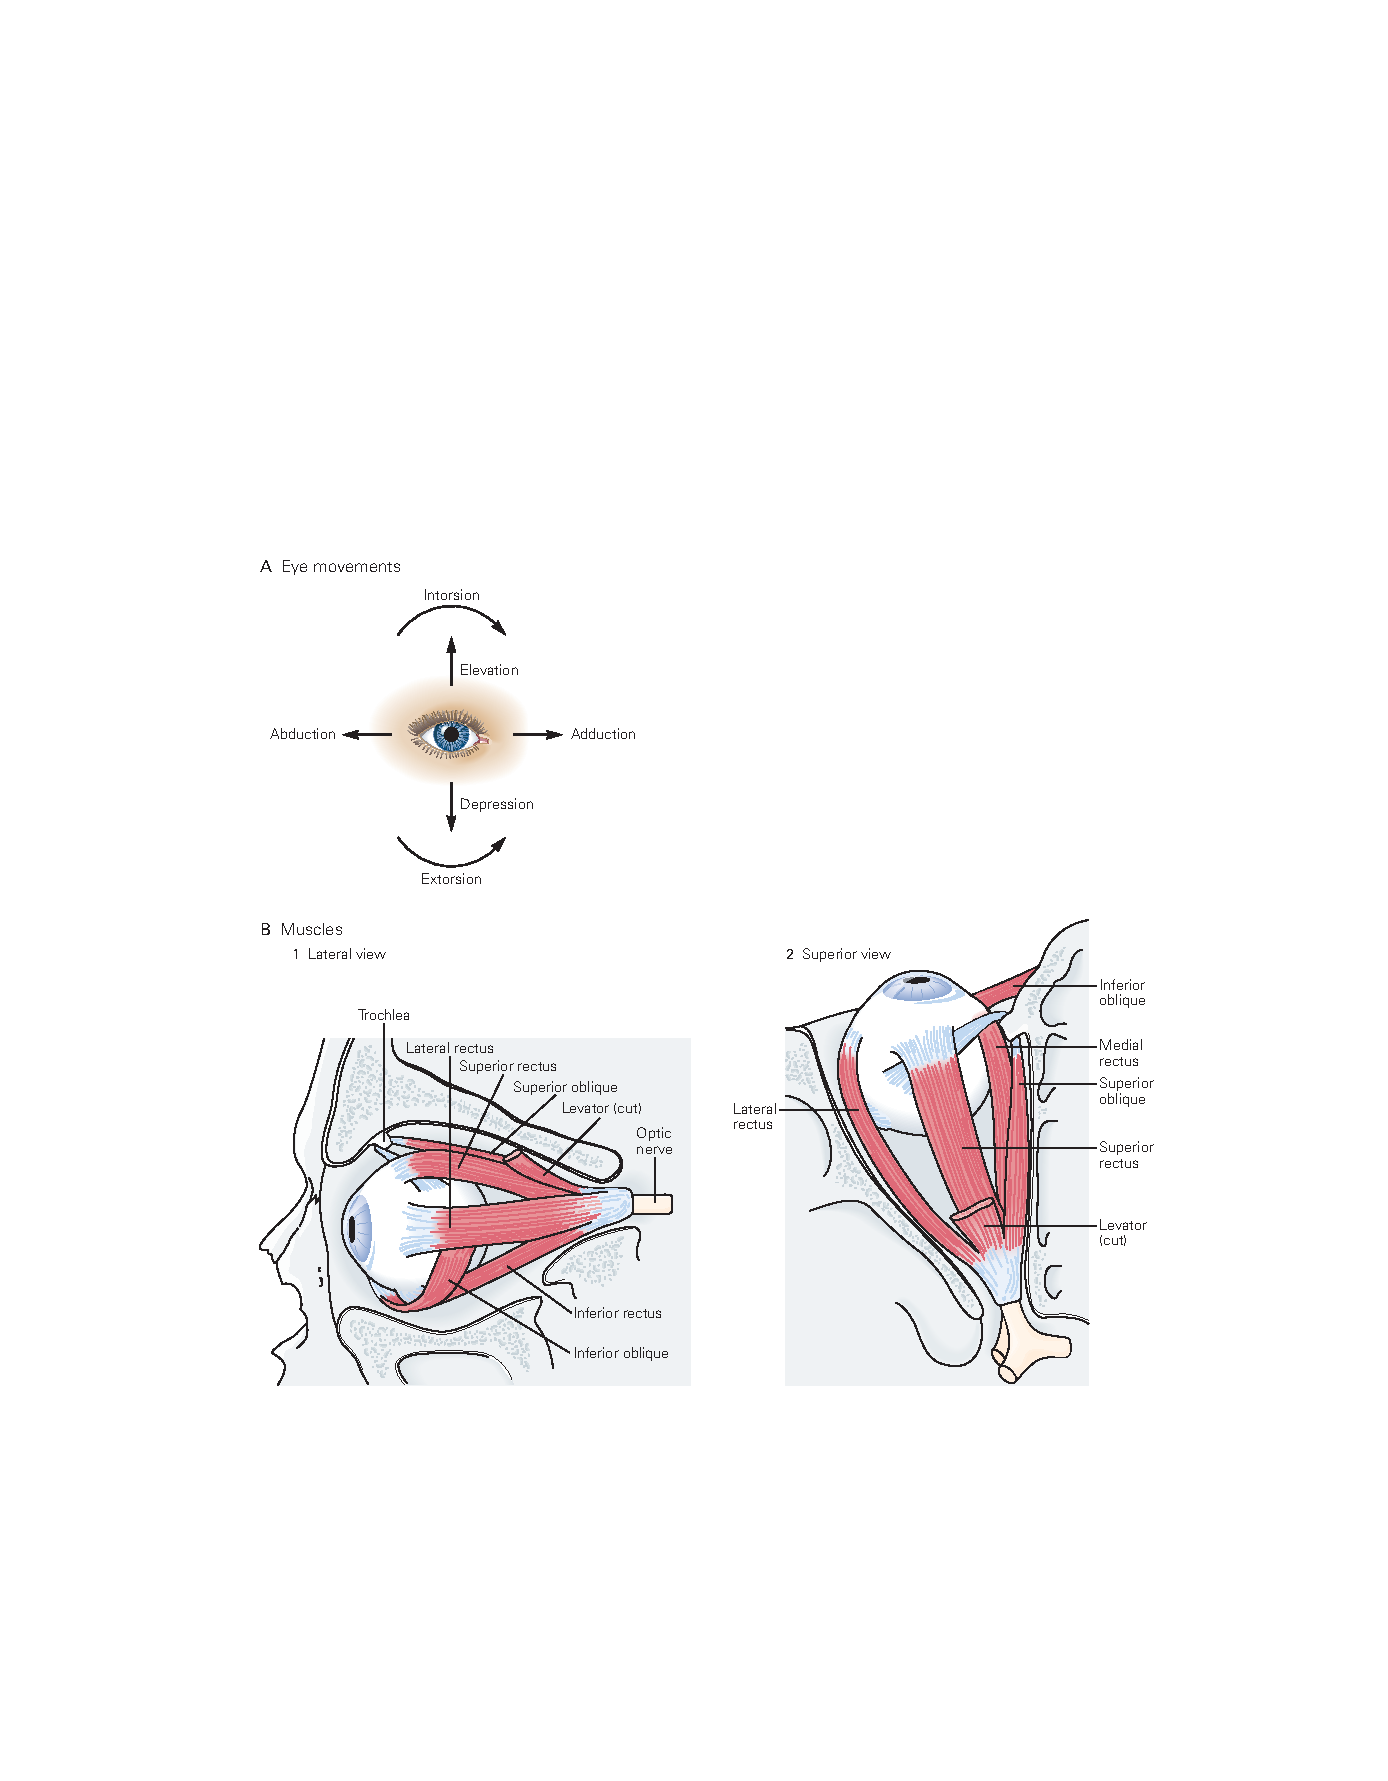
\includegraphics[width=0.85\linewidth]{chap35/fig_35_1}
	\caption{眼球运动的不同动作和控制它们的肌肉。 A. 左眼视图和眼球运动的三个维度。 B. 1. 左眼侧视图,眼眶壁被切除。 每块直肌都插入眼球赤道的前方,因此收缩使角膜向肌肉旋转。 相反,斜肌插入赤道后面,收缩使角膜旋转远离插入点。 上斜肌腱在插入眼球之前穿过滑车,滑车是眼眶鼻侧的骨滑轮。 上眼睑的提肌抬起眼睑。 2. 左眼俯视图,眼眶顶部和提肌被切除。 上直肌越过上斜肌并在地球上插入其前面。}
	\label{fig:35_1}
\end{figure}

大多数眼球运动是共轭的; 也就是说,双眼向同一方向移动。 这些眼球运动称为版本运动。 例如,在向右凝视时,右眼外展而左眼内收。 同样,如果右眼强行,左眼就会强行。 当你的目光由远变近时,眼睛会向相反的方向移动——双眼内收。 这些运动称为聚散运动。

\subsection{六块眼外肌形成三个主动-拮抗对}
每只眼睛由排列成三对激动剂-拮抗剂的六块眼外肌旋转(图 \ref{fig:35_1} B)。 四块直肌(外侧、内侧、上部和下部)有一个共同的起点,即位于眼眶顶点的 Zinn 环。 它们插入眼睛中心前面的眼睛表面或巩膜,因此上直肌抬高眼睛,下直肌压低眼睛。 下斜肌的起点在眼眶内侧壁上; 上斜肌的肌腱在插入眼球之前穿过滑车或滑车,因此它的有效起点也在眼眶的前内侧壁上。 斜肌插入眼睛中心的后方,因此上斜肌压低眼睛,下斜肌抬高眼睛。

每块肌肉都有双重插入。 离眼睛最远的肌肉部分插入软组织滑轮上,其余肌肉通过软组织滑轮到达眼睛。 当眼外肌收缩时,它们不仅会旋转眼睛,还会由于这些滑轮而改变其拉动方向。

眼外肌的动作由它们的几何形状和眼睛在眼眶中的位置决定。 内侧和外侧直肌水平旋转眼睛; 内直肌内收,而外直肌外展。 上直肌、下直肌和斜肌使眼睛在垂直方向和扭转方向上旋转。 上直肌和下斜肌抬高眼球,下直肌和上斜肌压低眼球。 上直肌和上斜肌进入眼睛,而下直肌和下斜肌外伸。

上直肌、下直肌和斜肌通常被称为旋垂直肌,因为它们产生垂直和扭转眼球旋转。 每次旋转的相对量取决于眼睛位置。 上直肌和下直肌在眼球外展时发挥最大垂直作用,即视线与肌肉牵拉方向平行时,而斜肌在眼球内收时发挥最大垂直作用(图 35) –2).



\subsection{两只眼睛的运动是协调的}
人类和其他正面眼睛的动物具有双眼视觉——两只眼睛的视野重叠。 这有助于立体视觉,即在三个维度上感知视觉场景的能力,以及深度感知。 同时,双眼视觉需要两只眼睛运动的精确协调,使两个中央凹始终对准感兴趣的目标。 对于大多数眼球运动,双眼必须以相同的量和相同的方向移动。 这在很大程度上是通过两只眼睛的眼部肌肉配对来实现的。

正如每块眼肌都与其在同一眼眶中的拮抗肌配对(例如,内侧和外侧直肌)一样,它也与在相同方向上移动对侧眼睛的肌肉配对。 例如,在向左扫视期间,左侧外直肌和右侧内直肌的耦合使双眼向左移动。 垂直肌的方向是这样的,每对由一根直肌和一根斜肌组成。 例如,左上直肌和右下斜肌在左眼注视时均使眼睛向上移动,而右下直肌和左上斜肌在右眼注视时均使眼球向下移动(表 35-1)。

\subsection{眼外肌由三个颅神经控制}

眼外肌受运动神经元组的支配,运动神经元的细胞体聚集在脑干的三个动眼神经核中(图 \ref{fig:35_3})。 
外直肌受外展神经(颅神经 VI)支配,外展神经的核位于第四脑室底部的桥脑中。 上斜肌受滑车神经(第四颅神经)支配,滑车神经核位于对侧中脑下丘水平。 (滑车神经得名于滑车,即上斜肌穿过的骨滑轮。)

\begin{figure}[htbp]
	\centering
	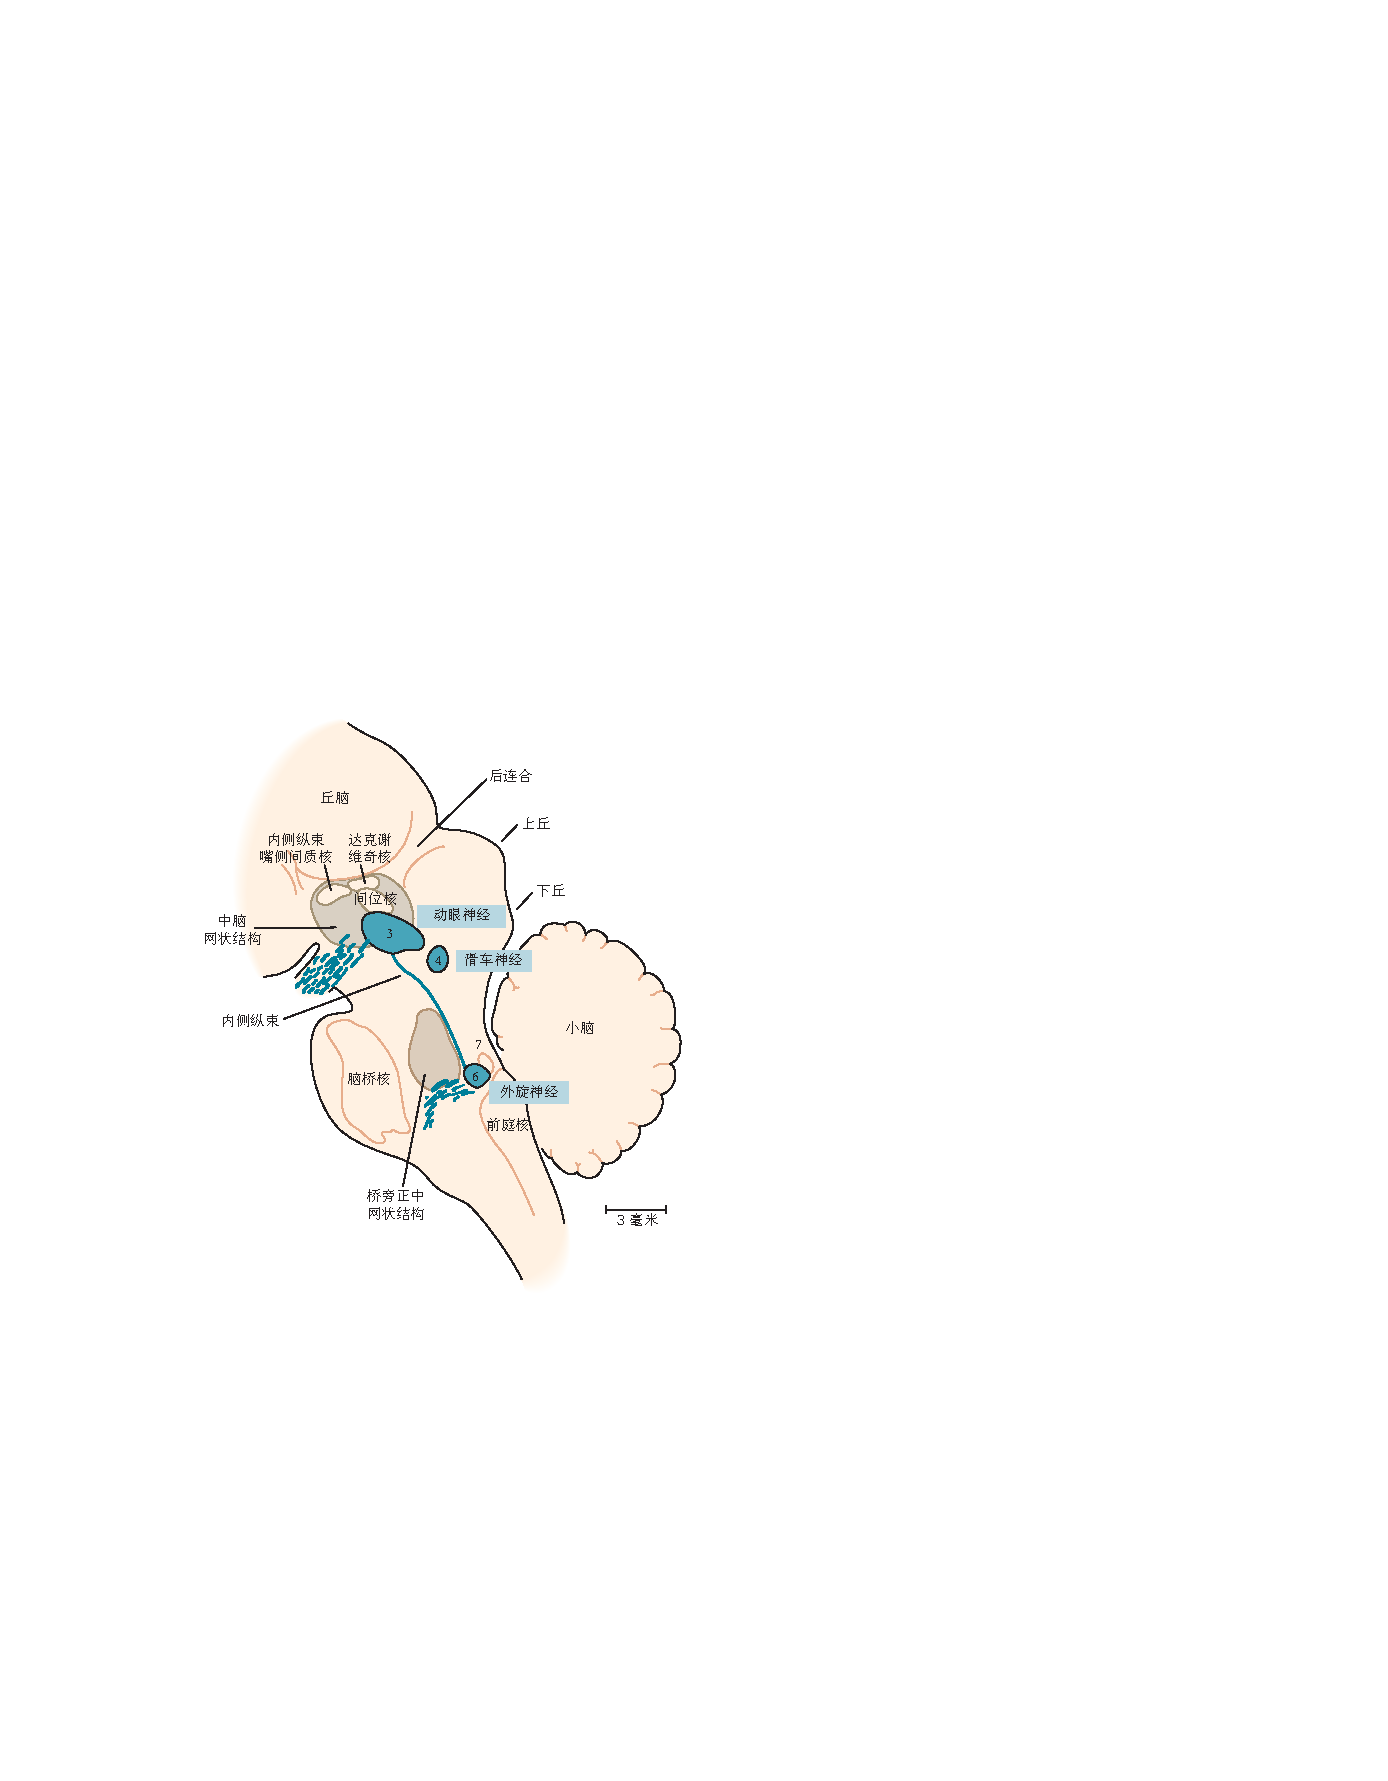
\includegraphics[width=0.5\linewidth]{chap35/fig_35_3}
	\caption{脑干中的动眼神经核。 细胞核显示在恒河猴的丘脑、脑桥、中脑和小脑的矢状旁切面中。 动眼神经核(颅神经 III)位于中脑中脑网状结构水平; 滑车核(神经 IV)略微位于尾部; 外展核(神经 VI)位于桥脑旁正中网状结构水平的脑桥,与面神经(VII)的束相邻。 与图 40–5 进行比较。 (缩写:iC,Cajal 间质核;iMLF,内侧纵束间质核;nD,Darkshevich 核;VN,前庭核。)(改编自 Henn、Hepp 和 Büttner-Ennever 1982。)}
	\label{fig:35_3}
\end{figure}

所有其他眼外肌——内侧、下部和上部直肌,以及下斜肌——由动眼神经(第 III 脑神经)支配,其核位于中脑上丘水平。 上直肌轴突穿过中线并加入对侧动眼神经。 因此,上直肌和上斜运动神经元支配它们各自在对侧的肌肉。 动眼神经还包含支配上眼睑提肌的纤维。 支配双眼睑的轴突细胞体位于中央尾核,这是动眼神经复合体中的单个中线结构。 最后,与动眼神经一起移动的是支配虹膜括约肌和睫状肌的副交感神经纤维,虹膜括约肌会收缩瞳孔,睫状肌会在从远到近的聚散运动过程中调整晶状体的曲率以聚焦眼睛,即调节过程。

瞳孔和眼睑也有交感神经支配,起源于同侧上胸段脊髓的中间外侧细胞柱。 这些神经元的纤维与上颈部的颈上神经节细胞形成突触。 这些节后细胞的轴突沿着颈动脉行进到海绵窦,然后进入眼眶。 交感神经瞳孔纤维支配虹膜扩张肌,导致瞳孔扩张,从而提供所谓的“战斗或逃跑”反应的瞳孔成分。 交感神经纤维还支配 Müller 的肌肉,这是上眼睑的二级提拉肌。 瞳孔扩张和眼睑抬高的交感神经控制是兴奋和交感神经超负荷的“睁大眼睛”表情的原因。


了解眼外肌活动的最佳方法是考虑特定神经损伤后仍然存在的眼球运动(方框 35-1)。

眼外肌产生的力由运动神经元的放电率和募集的运动单位数量决定。 与骨骼肌的运动单位(第 31 章)一样,眼球运动单位以固定顺序募集。 例如,当眼睛横向移动时,活跃的外展神经元数量及其个体放电率都会增加,从而增加外直肌收缩的强度。

\section{六种神经元控制系统保持目标的瞄准}
动眼神经核是高级大脑网络产生的所有类型眼球运动的最终共同目标。 Hermann Helmholtz 和其他 19 世纪的心理物理学家认为,眼球运动分析对于理解视觉感知至关重要,但他们假设所有眼球运动都是平滑的。 1890 年,埃德温·兰多特 (Edwin Landott) 发现,在阅读过程中,眼睛不会沿着一行文字平稳移动,而是会快速间歇性地移动,称为扫视(法语,jerks),每次扫视后都有一个短暂的停顿。

到 1902 年,雷蒙德·道奇 (Raymond Dodge) 概述了五种不同类型的眼球运动,它们将中央凹引导至视觉目标并将其保持在那里。 所有这些眼球运动都共享一个效应通路,该通路起源于脑干中的三个动眼神经核。

扫视眼球运动迅速将中央凹转移到新的视觉目标。

平滑的追踪运动将移动目标的图像保持在中央凹上。

聚散运动使眼睛朝相反的方向移动,因此无论距离多远,感兴趣的物体的图像都位于两个中央凹上。

前庭眼反射在短暂的头部运动期间稳定视网膜上的图像。

视动运动在持续的头部旋转或平移过程中稳定图像。


第六个系统,即注视系统,在头部不动时通过主动抑制眼球运动使眼睛保持静止。 视动系统和前庭系统在第 27 章中讨论。我们在这里考虑其他四个系统。

\subsection{主动固定系统将中央凹固定在固定目标上}
当眼睛静止时,视力最准确。 当我们检查感兴趣的对象时,凝视系统会主动防止眼睛移动。 当我们做一些不需要视觉的事情时,比如心算,它就不会那么积极地抑制运动。 注视系统障碍的患者——例如,无法抑制眼球扫视运动(视阵挛)的患者——视力不佳不是因为他们的视敏度不足,而是因为他们不能保持眼睛足够静止以使视觉系统正常工作。

\subsection{扫视系统将中央凹指向感兴趣的对象}

我们的眼睛通过一系列非常快速的扫视探索世界,这些扫视将中央凹从一个注视点移动到另一个注视点(第 25 章)(图 \ref{fig:35_5})。 眼跳使我们能够快速扫描环境并阅读。 
高度刻板,他们有一个标准的波形,眼速度有一个平滑的增加和减少。 眼跳也非常快,在几分之一秒内以高达每秒 900° 的角速度发生(图 \ref{fig:35_6} A)。 
眼跳的速度仅由其大小决定。 我们可以自愿改变眼跳的幅度和方向,但不能改变眼跳的速度,尽管疲劳、药物或病理状态会减慢眼跳。

\begin{figure}[htbp]
	\centering
	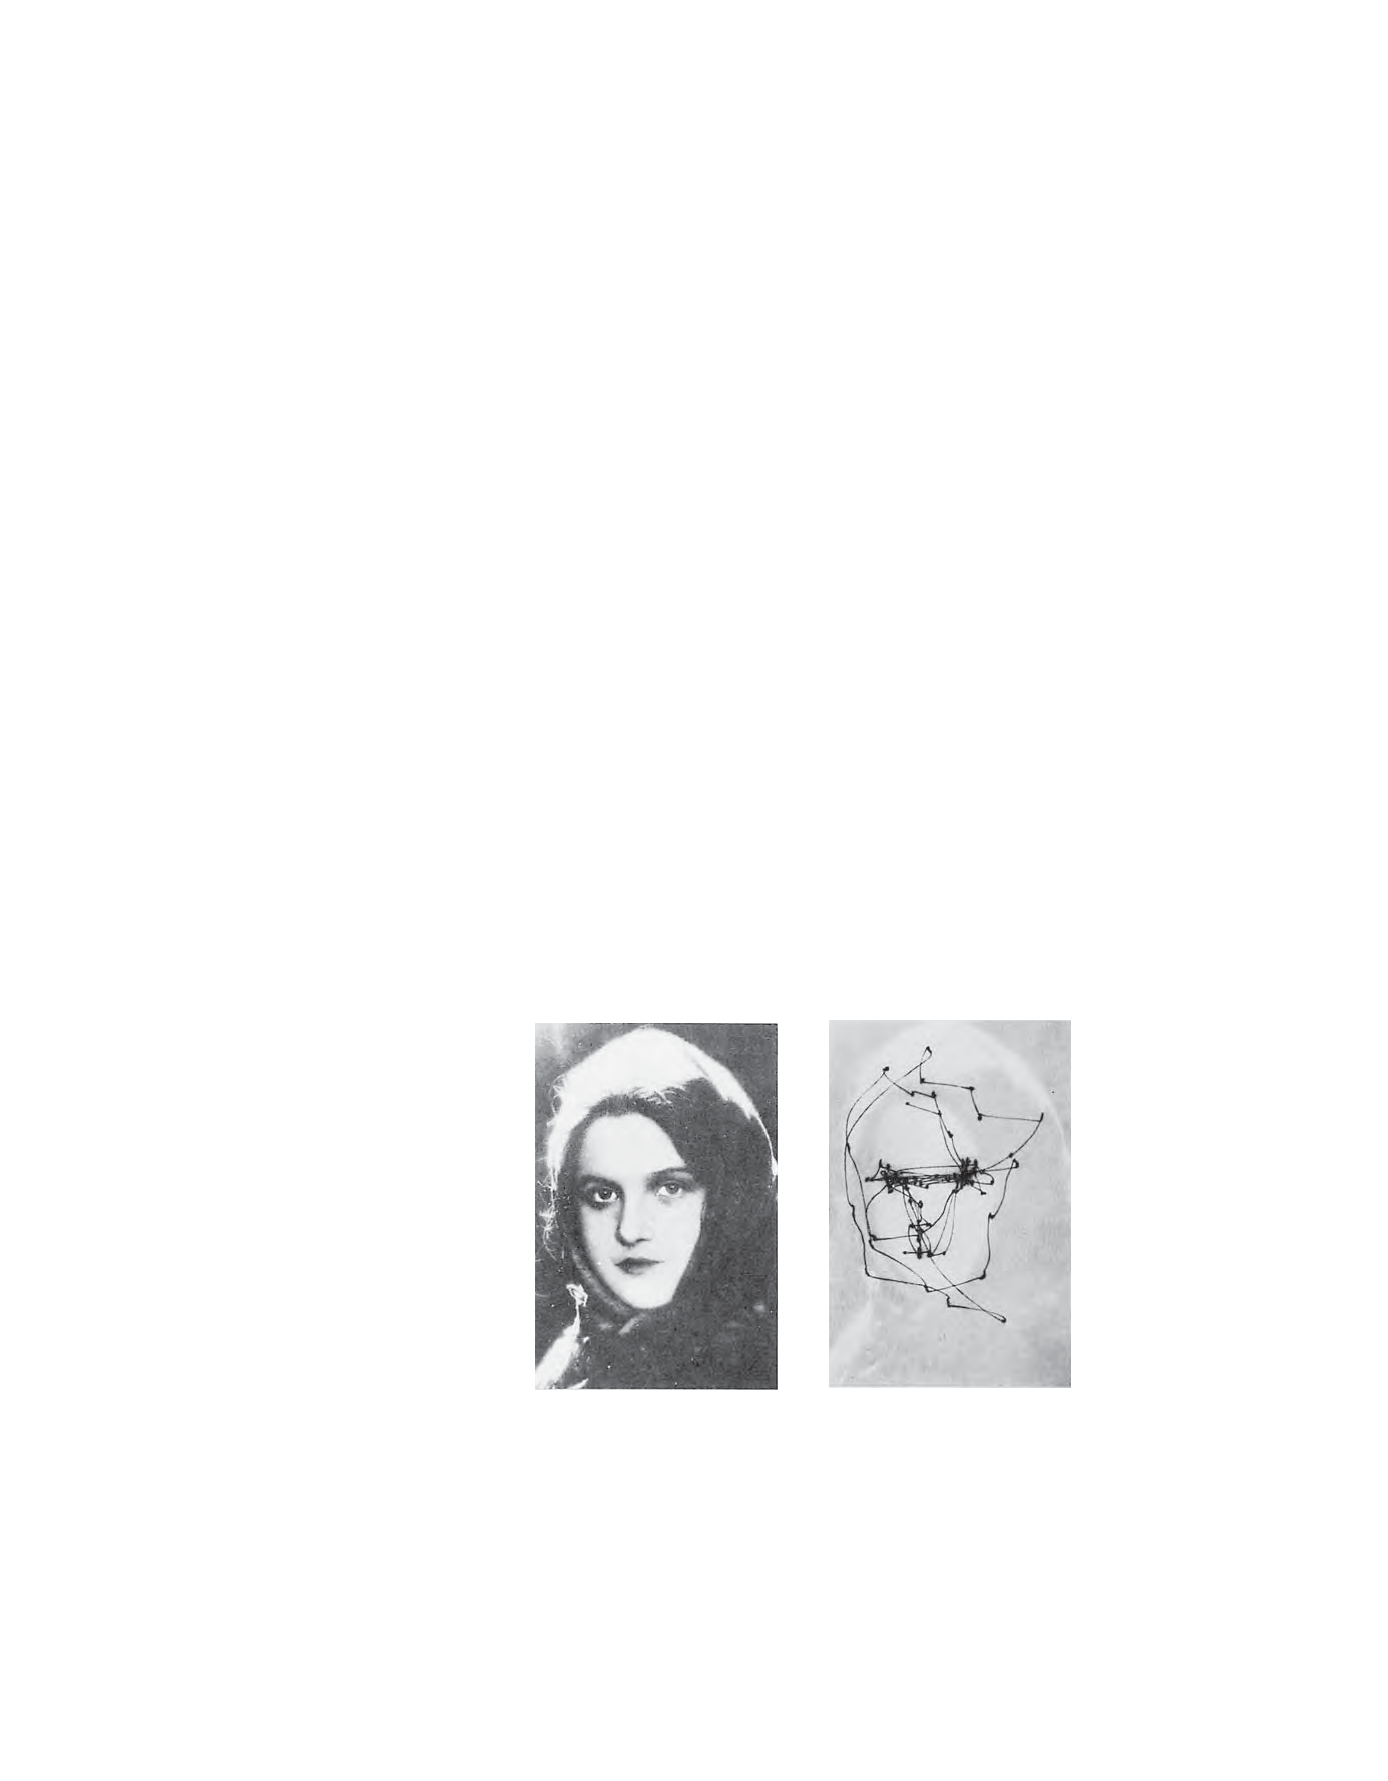
\includegraphics[width=0.4\linewidth]{chap35/fig_35_5}
	\caption{眼球运动跟踪关注对象的轮廓。 观察者注视一张女性照片 1 分钟。 然后将得到的眼睛位置叠加在图片上。 如图所示,观察者专注于脸部的某些特征,在女人的眼睛和嘴巴上逗留(注视),并在中间位置花费较少的时间。 注视点之间的快速移动是眼跳。 (经许可转载自 Yarbus 1967。)}
	\label{fig:35_5}
\end{figure}

\begin{figure}[htbp]
	\centering
	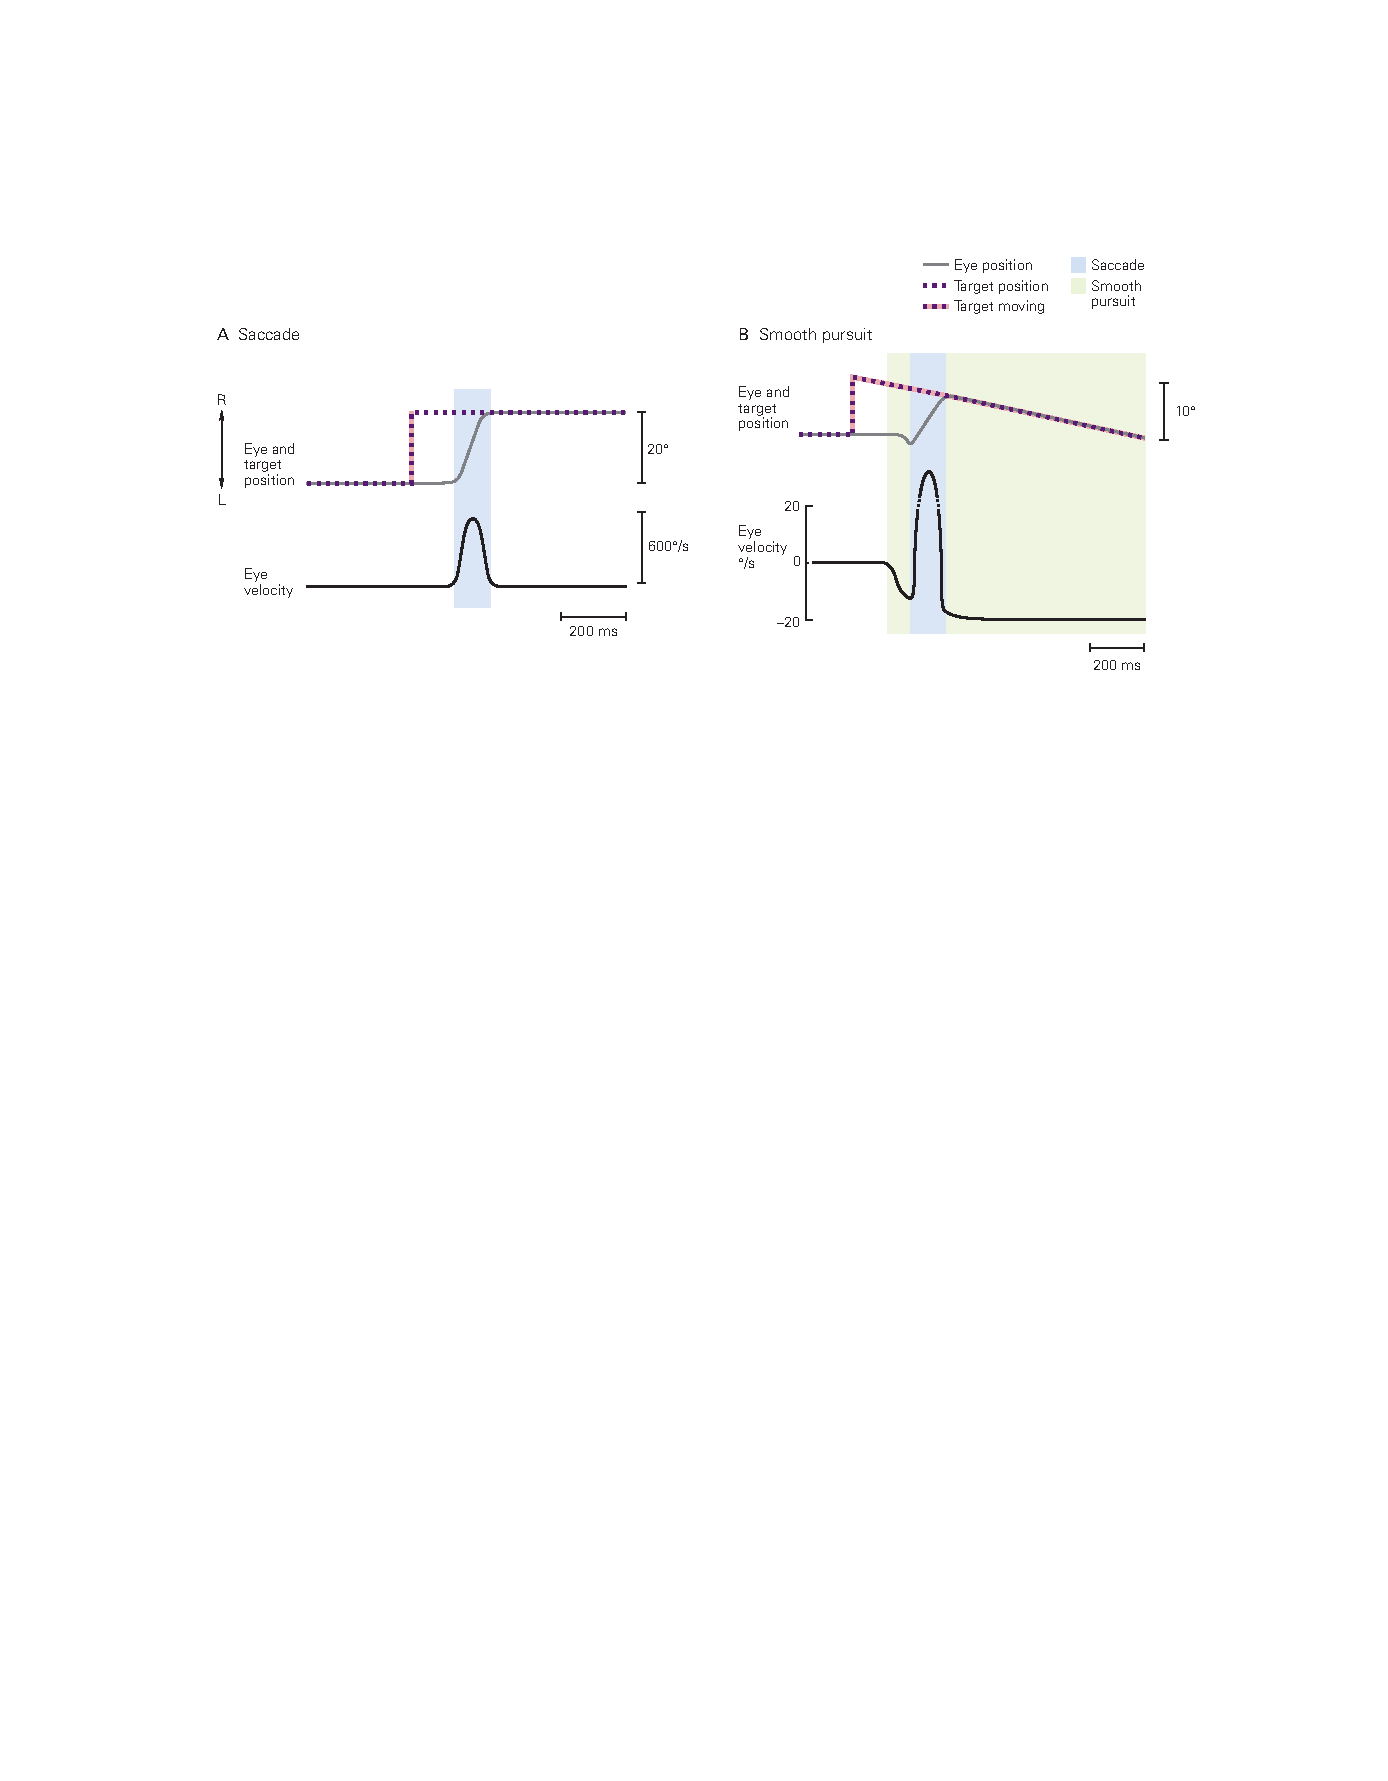
\includegraphics[width=0.9\linewidth]{chap35/fig_35_6}
	\caption{扫视和平滑的眼球运动。 眼睛位置、目标位置和眼睛速度随时间绘制。 A. 人体扫视。 在情节的开始,眼睛在目标上(代表眼睛和目标位置的轨迹是叠加的)。 突然,目标向右跳,在 200 毫秒内,眼睛移动将目标带回中央凹。 请注意平滑、对称的速度曲线。 因为眼球运动是眼球在眼眶内的旋转,所以用旋转角度来描述。 类似地,视野中的物体通过它们对着眼睛的弧度来描述。 从手臂的长度看,拇指所夹的角度大约为 1°。 因此,从拇指的一个边缘到另一个边缘的扫视穿过 1° 的弧度。 (缩写:L,左;R,右。) B. 人类平稳的追求。 在这个例子中,受试者被要求对一个目标进行扫视,该目标从注视中心跳开,然后慢慢移回中心。 在位置和速度轨迹中看到的第一个运动是与目标运动方向相同的平滑追踪运动。 在开始扫视之前,眼睛会短暂地离开目标,因为追踪系统的延迟比扫视系统的延迟短。 平滑追踪系统由目标向回注视中心移动激活,扫视调整眼睛的位置以捕捉目标,此后平滑追踪使眼睛保持在目标上。 扫视速度的记录被剪裁,以便运动可以显示在追逐运动的尺度上,比扫视慢一个数量级。}
	\label{fig:35_6}
\end{figure}

通常,没有时间让视觉反馈来修改扫视的过程; 相反,对运动方向和/或幅度的修正是在连续的扫视过程中进行的。 准确的扫视不仅可以针对视觉目标,还可以针对声音、触觉刺激、空间位置的记忆,甚至口头命令(例如,“向左看”)。

当进行扫视时,控制注视的高级大脑中枢神经元的活动仅指定所需的眼睛位置变化(例如,当前注视右侧 20°,通常基于视野中的目标位置)。 对于要进行的眼球运动,必须将该位置信号转换为眼肌信号,以执行所需的速度并改变眼球位置。 
我们可以通过考虑扫视期间动眼神经元的活动来说明注视系统如何产生眼球运动(图 \ref{fig:35_7} A)。 
要将眼睛快速移动到眼眶中的新位置并保持在那里,必须克服两个被动力:眼眶组织的弹力,它倾向于将眼睛恢复到中心位置,以及与速度相关的粘性力 反对快速运动。 因此,眼球运动的运动信号必须包括抵消弹性力的位置分量和克服眼眶粘性并将眼睛快速移动到新位置的速度分量。

\begin{figure}[htbp]
	\centering
	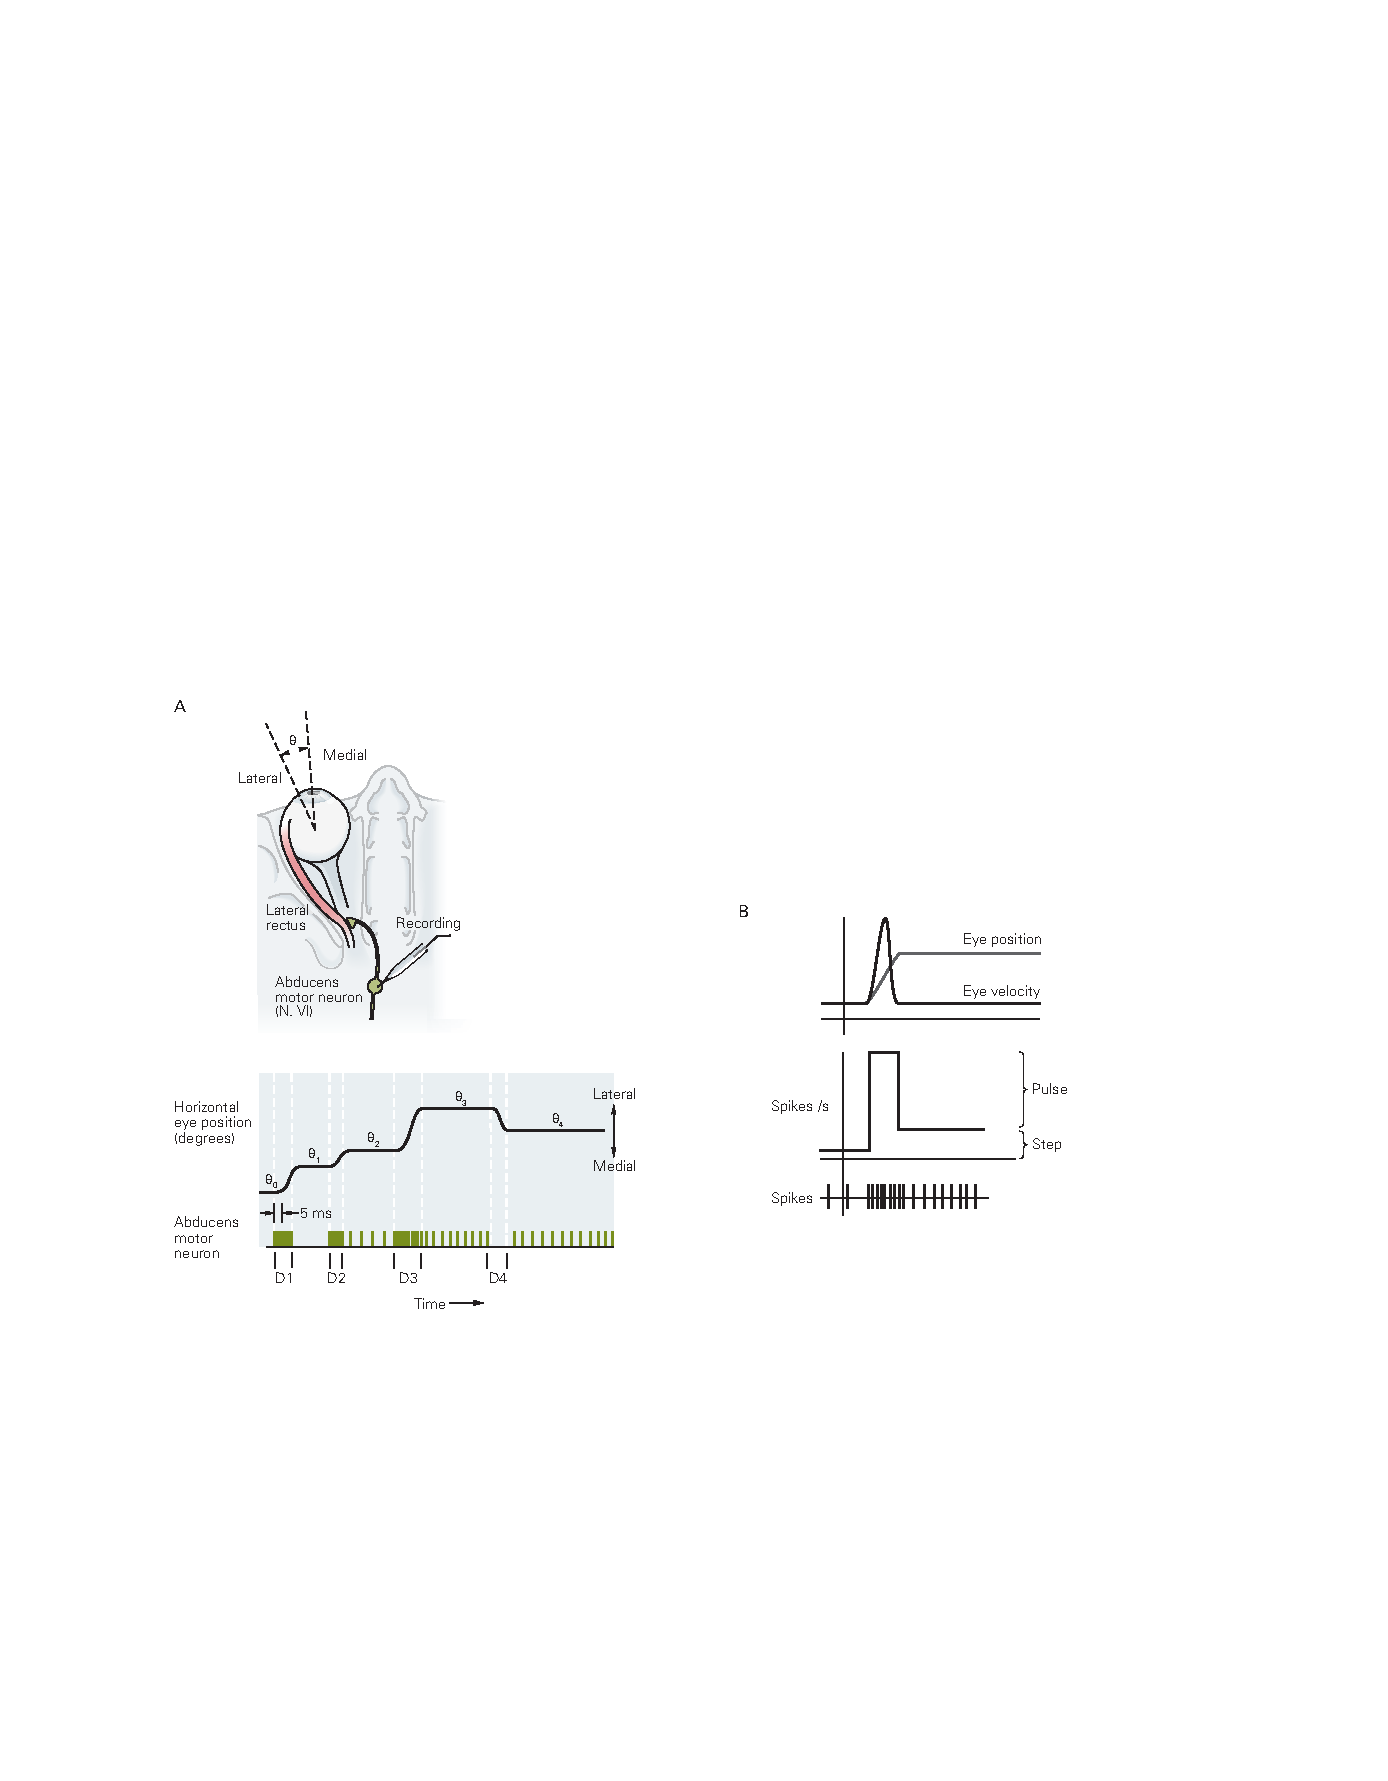
\includegraphics[width=0.5\linewidth]{chap35/fig_35_7}
	\caption{动眼神经元发出眼睛位置和速度的信号。 A. 记录来自猴子的外展神经元。 当眼睛位于眼眶内侧时,细胞是无声的(位置 θ0)。 当猴子进行横向扫视时,会有一阵放电 (D1),但在新位置 (θ1),眼睛仍然太靠内侧,细胞无法持续放电。 在下一个扫视期间,有一个突发 (D2),在新位置 (θ2),有一个与强直位置相关的放电。 在下一次扫视 (D3) 之前和期间,当眼睛处于新位置 (θ3) 时,再次出现活动脉冲和更高的强直放电。 当眼睛向内侧移动时,在扫视 (D4) 期间会有一段静止期,即使眼睛最终位于与强直性放电相关的位置 (θ4)。 (改编自 Fuchs 和 Luschei 1970。)B. 扫视与一个活动步骤相关,它表示眼睛位置的变化,以及一个活动脉冲,它表示眼睛速度。 与眼睛位置和速度相对应的神经活动被说明为一串单独的尖峰和瞬时发射率(每秒尖峰)的估计。}
	\label{fig:35_7}
\end{figure}

这种眼睛位置和速度信息由动眼神经元的放电频率编码。 进行扫视时,神经元的放电率会随着眼动速度的增加而迅速增加; 这称为扫视脉冲(图 \ref{fig:35_7}B)。 该脉冲的频率决定了眼跳的速度,而脉冲的长度控制了眼跳的持续时间,从而控制了眼跳的幅度。 当扫视完成并且眼睛达到目标时,必须有一个新的强直输入水平输入到眼眶肌肉,以适应该眼眶位置的弹性恢复力。 扫视前后强直放电率的这种差异称为扫视步长(图 \ref{fig:35_7}B)。 如果步幅大小与脉冲不匹配,则眼睛在扫视后会偏离目标。 如后所述,脉冲和阶跃是由不同的脑干结构产生的。

\section{扫视的运动环路位于脑干}
\subsection{桥脑网状结构产生水平扫视}
水平眼跳的神经元信号起源于桥脑旁正中网状结构,与它投射到的外展核相邻(图 \ref{fig:35_8} A)。 
桥脑旁正中网状结构包含一系列突发神经元,可产生扫视脉冲。 这些细胞在同侧眼跳之前和期间以高频放电(朝向与放电神经元相同的一侧),并且它们的活动类似于动眼神经元放电的脉冲分量(图 \ref{fig:35_7}B)。

\begin{figure}[htbp]
	\centering
	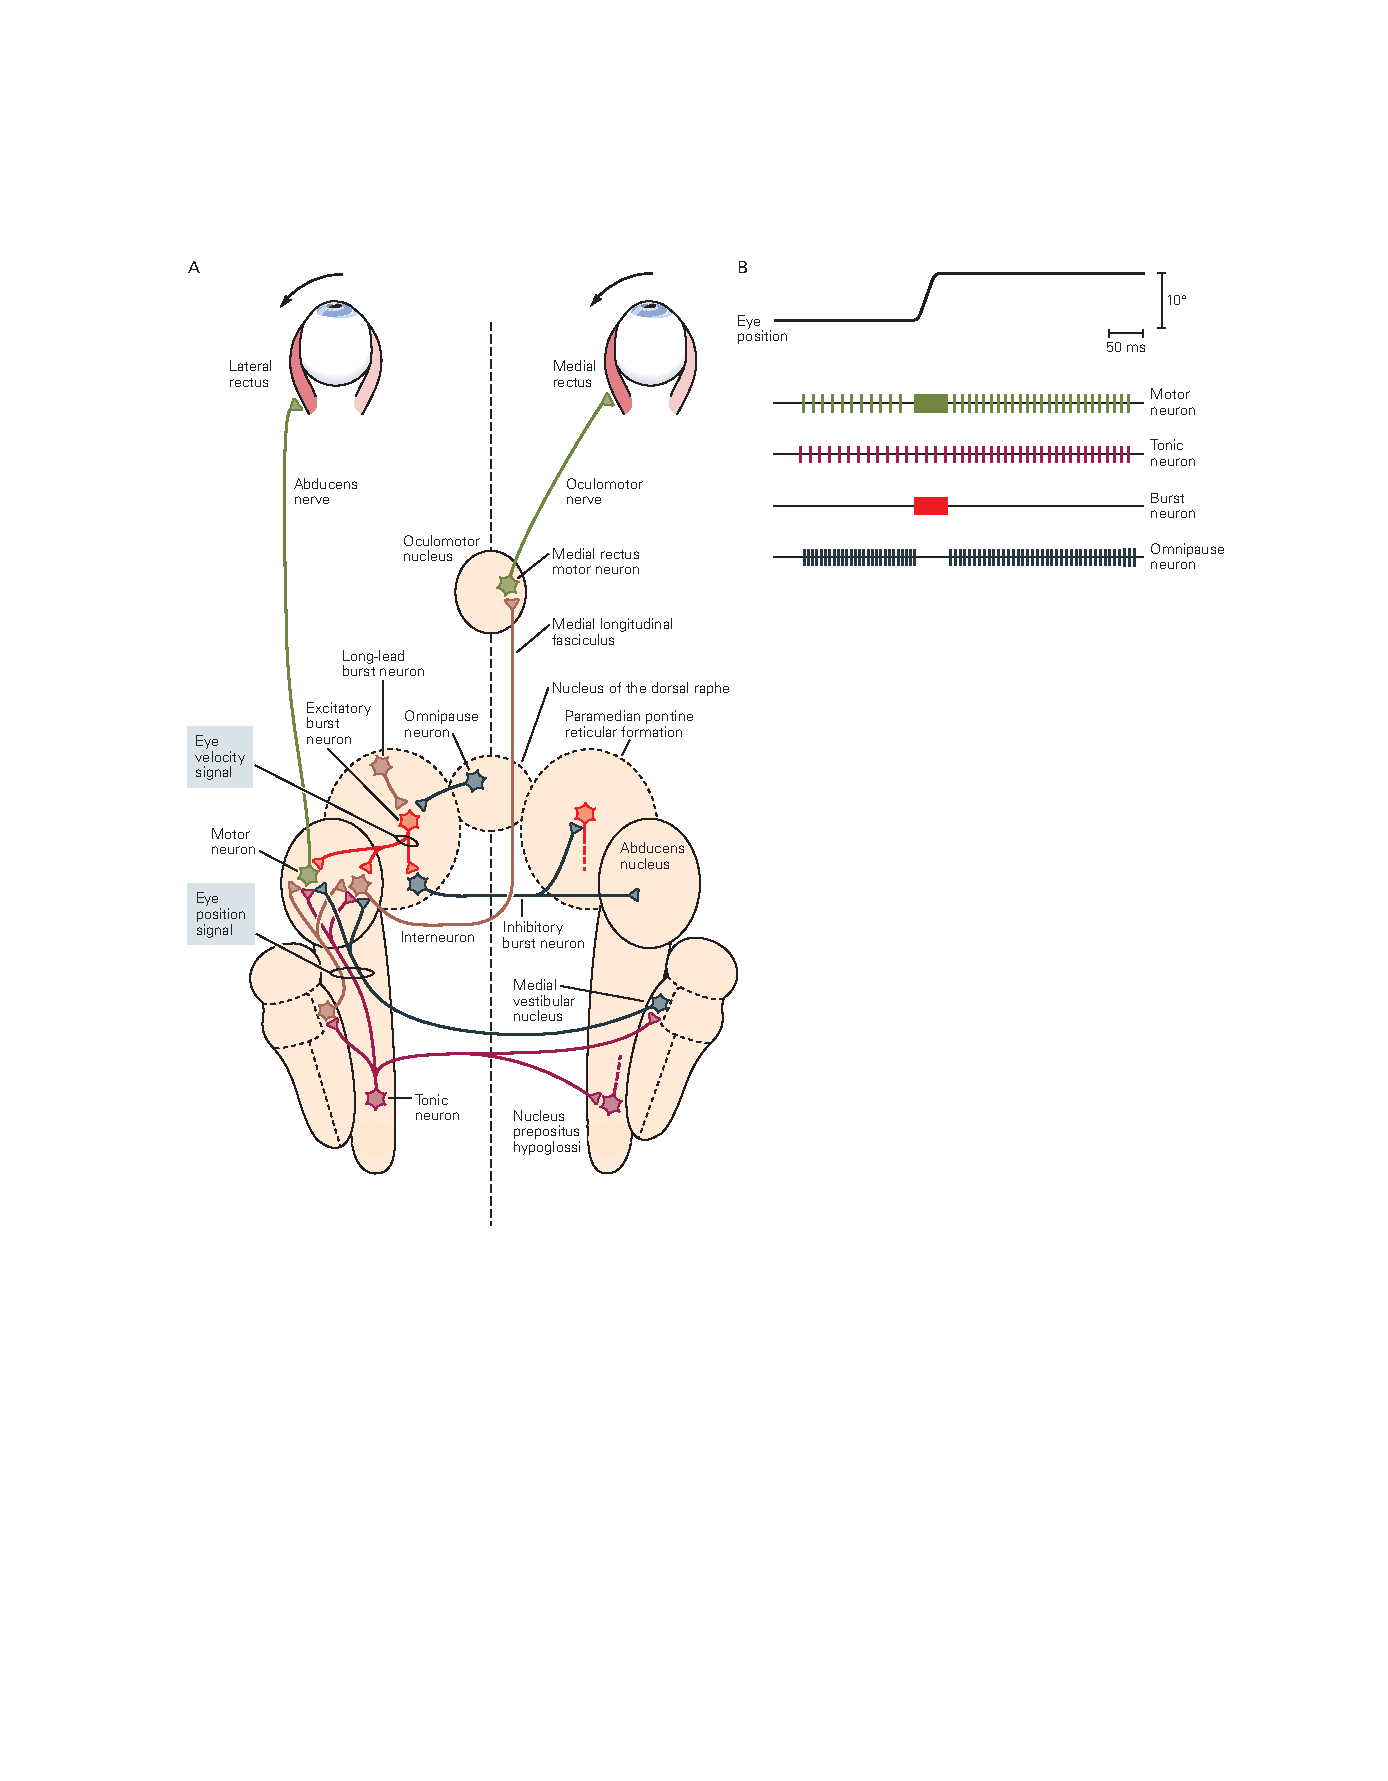
\includegraphics[width=0.95\linewidth]{chap35/fig_35_8}
	\caption{水平扫视的脑干运动电路。 
		A. 眼动速度分量。 长导联爆发神经元将信号从更高的中心传递到兴奋性爆发神经元。 眼速度分量来自桥脑旁正中网状结构中的兴奋性爆发神经元,该神经元与外展核中的运动神经元和中间神经元形成突触。 外展运动神经元投射到同侧外直肌,而中间神经元通过穿过中线并在内侧纵束中上升的轴突投射到对侧内直肌运动神经元。 兴奋性爆发神经元也驱动抑制对侧外展运动神经元和兴奋性爆发神经元的同侧抑制性爆发神经元。 眼睛位置组件。 该成分来自一个神经整合器,该整合器包含分布在脑干两侧的前庭内侧核和舌下前核的神经元。 这些神经元接收来自兴奋性爆发神经元的速度信号,并将该速度信号整合为位置信号。 位置信号激发同侧外展神经元并抑制对侧外展神经元。 (灰色神经元是抑制性的;所有其他神经元都是兴奋性的。垂直虚线表示脑干的中线。) B. 不同的神经元为水平扫视提供不同的信息。 运动神经元提供位置和速度信号。 强直神经元 (nucleus prepositus hypoglossi) 只发出眼睛位置的信号。 兴奋性爆发神经元(桥脑旁正中网状结构)仅发出眼动速度信号。 除眼跳之前、期间和之后的瞬间外,全暂停神经元以高速率放电。}
	\label{fig:35_8}
\end{figure}

有几种类型的突发神经元(图 \ref{fig:35_8}B)。 中导兴奋性爆发神经元与同侧外展核中的运动神经元和中间神经元直接兴奋连接。 长导联爆发神经元驱动中导联爆发细胞并接收来自更高中心的兴奋性输入。 抑制性爆发神经元抑制对侧外展神经元和对侧兴奋性爆发神经元的活动,并且自身被中导爆发神经元兴奋。

第二类桥脑细胞,全停期神经元,除了在扫视时会持续放电; 在所有眼跳之前和期间不久,放电停止(图 \ref{fig:35_8}B)。 Omnipause 神经元位于中线背侧中缝的核内(图 \ref{fig:35_8}A)。 它们是 GABA 能(γ-氨基丁酸)抑制性神经元,投射到对侧桥脑和中脑爆发神经元。 全暂停神经元的电刺激会阻止眼跳,当刺激停止时眼跳会恢复。 进行眼跳需要同时激发突发神经元和抑制全暂停细胞; 这为系统提供了额外的稳定性,这样不需要的扫视就很少见了。

如果运动神经元只接收来自爆发细胞的信号,眼睛会在扫视后漂移回到起始位置,因为没有新的位置信号来保持眼睛抵抗弹性恢复力。 需要适当的强直神经支配才能将眼睛保持在新的眼眶位置。 这种强直位置信号,即扫视步,可以通过积分数学过程的神经等价物从速度突发信号生成。 可以通过相对于时间对位置进行微分来计算速度; 相反,可以通过相对于时间对速度进行积分来计算位置。

对于水平眼球运动,速度信号的神经整合由内侧前庭核和舌下核前位核(图 \ref{fig:35_8}A)与小脑的绒球共同完成。 正如预期的那样,这些区域受损的动物会进行正常的水平扫视,但扫视后眼睛会漂移回中间位置。 此外,水平扫视爆发的整合需要通过连合连接协调双侧舌下前位核和内侧前庭核。 因此,这些连接的中线损伤也会导致神经整合器失效。

桥脑旁正中网状结构中的中导突发神经元和内侧前庭核和舌下核前位核的神经元投射到同侧外展核,并分别传递运动信号的脉冲和步进分量。 外展核中的两个神经元群接收到这个信号。 一个是一组运动神经元,支配同侧外直肌。 第二组由中间神经元组成,其轴突穿过中线并在内侧纵束中上升到位于动眼神经核中的对侧内侧直肌的运动神经元(图 \ref{fig:35_8}A)。

因此,内直肌运动神经元不直接接收脉冲和步进信号。 这种布置允许在水平扫视和其他共轭眼球运动期间精确协调双眼的相应运动。 内侧纵束对中风和多发性硬化症的易感性使其在临床上很重要。

几个小脑结构在扫视运动信号的校准中起着重要作用。 首先,背蚓部的动眼神经部分通过尾部顶核起作用,控制脉冲的持续时间,从而控制眼跳的准确性。 顶核在反向扫视开始时增加扫视速度,并有助于制动同向扫视以结束扫视。 其次,前庭小脑的绒球和副绒球校准神经整合器以确保步进与脉冲正确匹配,以便在每次扫视后将眼睛保持在新位置。


\subsection{中脑网状结构中产生垂直扫视}
在中脑网状结构中的内侧纵束的头端间质核中发现了负责垂直眼跳的爆发神经元(图 \ref{fig:35_3})。 垂直和扭转神经整合在附近的 Cajal 间质核中进行。 脑桥和中脑系统共同参与斜扫视的产生,斜扫视既有水平分量也有垂直分量。

纯垂直眼跳需要中脑网状结构两侧的活动,两侧之间的交流通过后连合发生。 水平和垂直扫视没有单独的全暂停神经元; 桥脑 omnipause 细胞抑制桥脑和中脑爆发神经元。

\subsection{脑干病变导致眼球运动的特征性缺陷}
我们现在可以了解不同的脑干病变如何引起特征性综合征。 包括桥脑旁正中网状结构在内的病变导致双眼的同侧水平凝视麻痹,但保留反向和垂直扫视。 外展核的损伤具有类似的效果,因为外展运动神经元和中间神经元都受到影响。 包括中脑凝视中枢在内的病变会导致垂直凝视麻痹。 某些神经系统疾病会导致突发神经元退化并损害其功能,从而导致眼跳逐渐减慢。

内侧纵束的损伤使内侧直肌运动神经元与外展中间神经元断开(图 \ref{fig:35_8}A)。 因此,在共轭水平眼球运动期间,例如扫视和追逐,外展眼正常移动,但另一只眼内收受阻。 尽管在倒转运动中存在这种麻痹,但内直肌通常在聚散运动中正常发挥作用,因为聚散的运动神经元位于中脑,这将在后面讨论。 这种称为核间性眼肌麻痹的综合征是脑干中风或多发性硬化症等脱髓鞘疾病的结果。

由于扫视爆发的正常终止失败,小脑顶核的损伤会导致同侧扫视超过其目标(超速扫视)。 Contraversive saccades undershoot their targets (hypometric saccades)。 相应地,对动眼蚓部的损伤会抑制顶核并导致低度同向扫视。 这可能是由于额外未能补偿眼眶组织的位置相关被动力。


\section{扫视通过上丘由大脑皮层进行控制}
桥脑和中脑突发回路提供驱动眼外肌进行眼跳所必需的运动信号。 然而,在高等哺乳动物中,眼球运动最终是由认知行为驱动的。 何时何地进行行为上重要的扫视的决定通常在大脑皮层中做出。 
皮质和皮质下区域的网络通过上丘控制眼跳系统(图 \ref{fig:35_9})。

\begin{figure}[htbp]
	\centering
	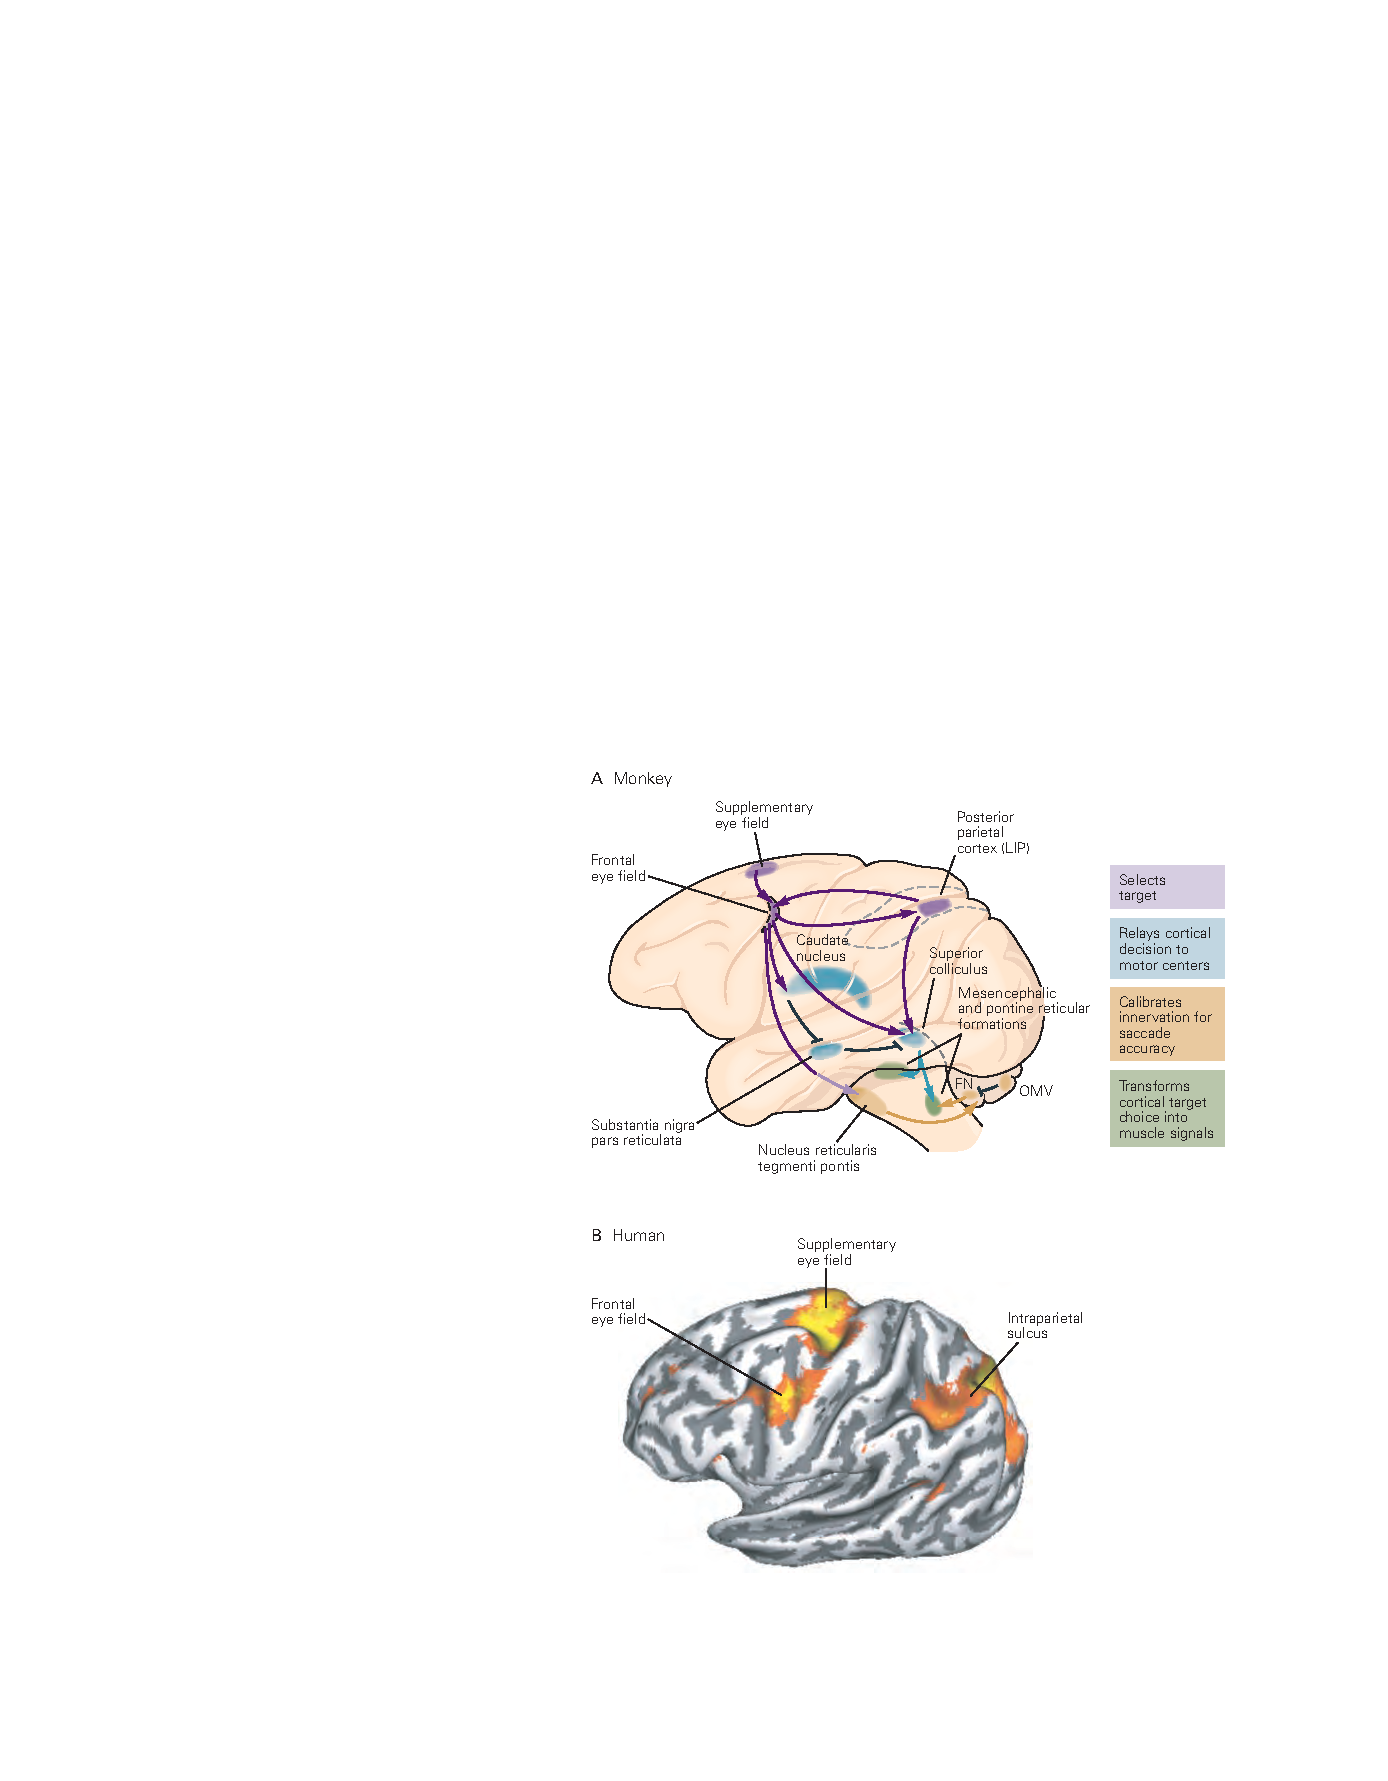
\includegraphics[width=0.6\linewidth]{chap35/fig_35_9}
	\caption{用于眼跳的皮层通路。 A. 在猴子身上,脑干中的眼跳发生器接收来自上丘的命令。 该命令通过脑桥和中脑突发回路传递,提供驱动眼外肌进行眼跳的运动信号。 丘接收来自额叶眼区和外侧顶内区 (LIP) 的直接兴奋性投射和来自黑质的抑制性投射。 黑质被尾状核抑制,而尾状核又被额叶眼场兴奋。 因此,前额眼场直接刺激丘,并通过刺激抑制黑质的尾状核,间接将其从黑质的抑制中释放出来。 小脑的动眼蚓 (OMV) 通过顶核 (FN) 起作用,校准爆发以保持扫视准确。 B. 人脑的横向扫描显示在扫视期间激活的皮质区域。 (改编自 Curtis 和 Connolly 2008。)}
	\label{fig:35_9}
\end{figure}


\subsection{上丘将视觉和运动信息整合到脑干的动眼神经信号中}
中脑的上丘是一个主要的视觉运动整合区域,是非哺乳动物脊椎动物视顶盖的哺乳动物同系物。 它可分为两个功能区域:浅层和中深层。

三个表层接收来自视网膜的直接输入和来自代表整个对侧视觉半场的纹状皮层的投射。 表层的神经元对视觉刺激有反应。 在猴子中,当动物准备对细胞感受野中的刺激进行扫视时,这些与视觉相关的神经元中有一半的反应在数量上得到增强。 此增强功能特定于扫视。 如果猴子注意到刺激而不进行扫视——例如,通过手部运动来响应亮度变化——神经元的反应不会增强。 
上丘表层的神经元在功能上排列在视野的视网膜专题图中,其中最靠近中央凹的视野代表占据最大区域(图 \ref{fig:35_10})。

\begin{figure}[htbp]
	\centering
	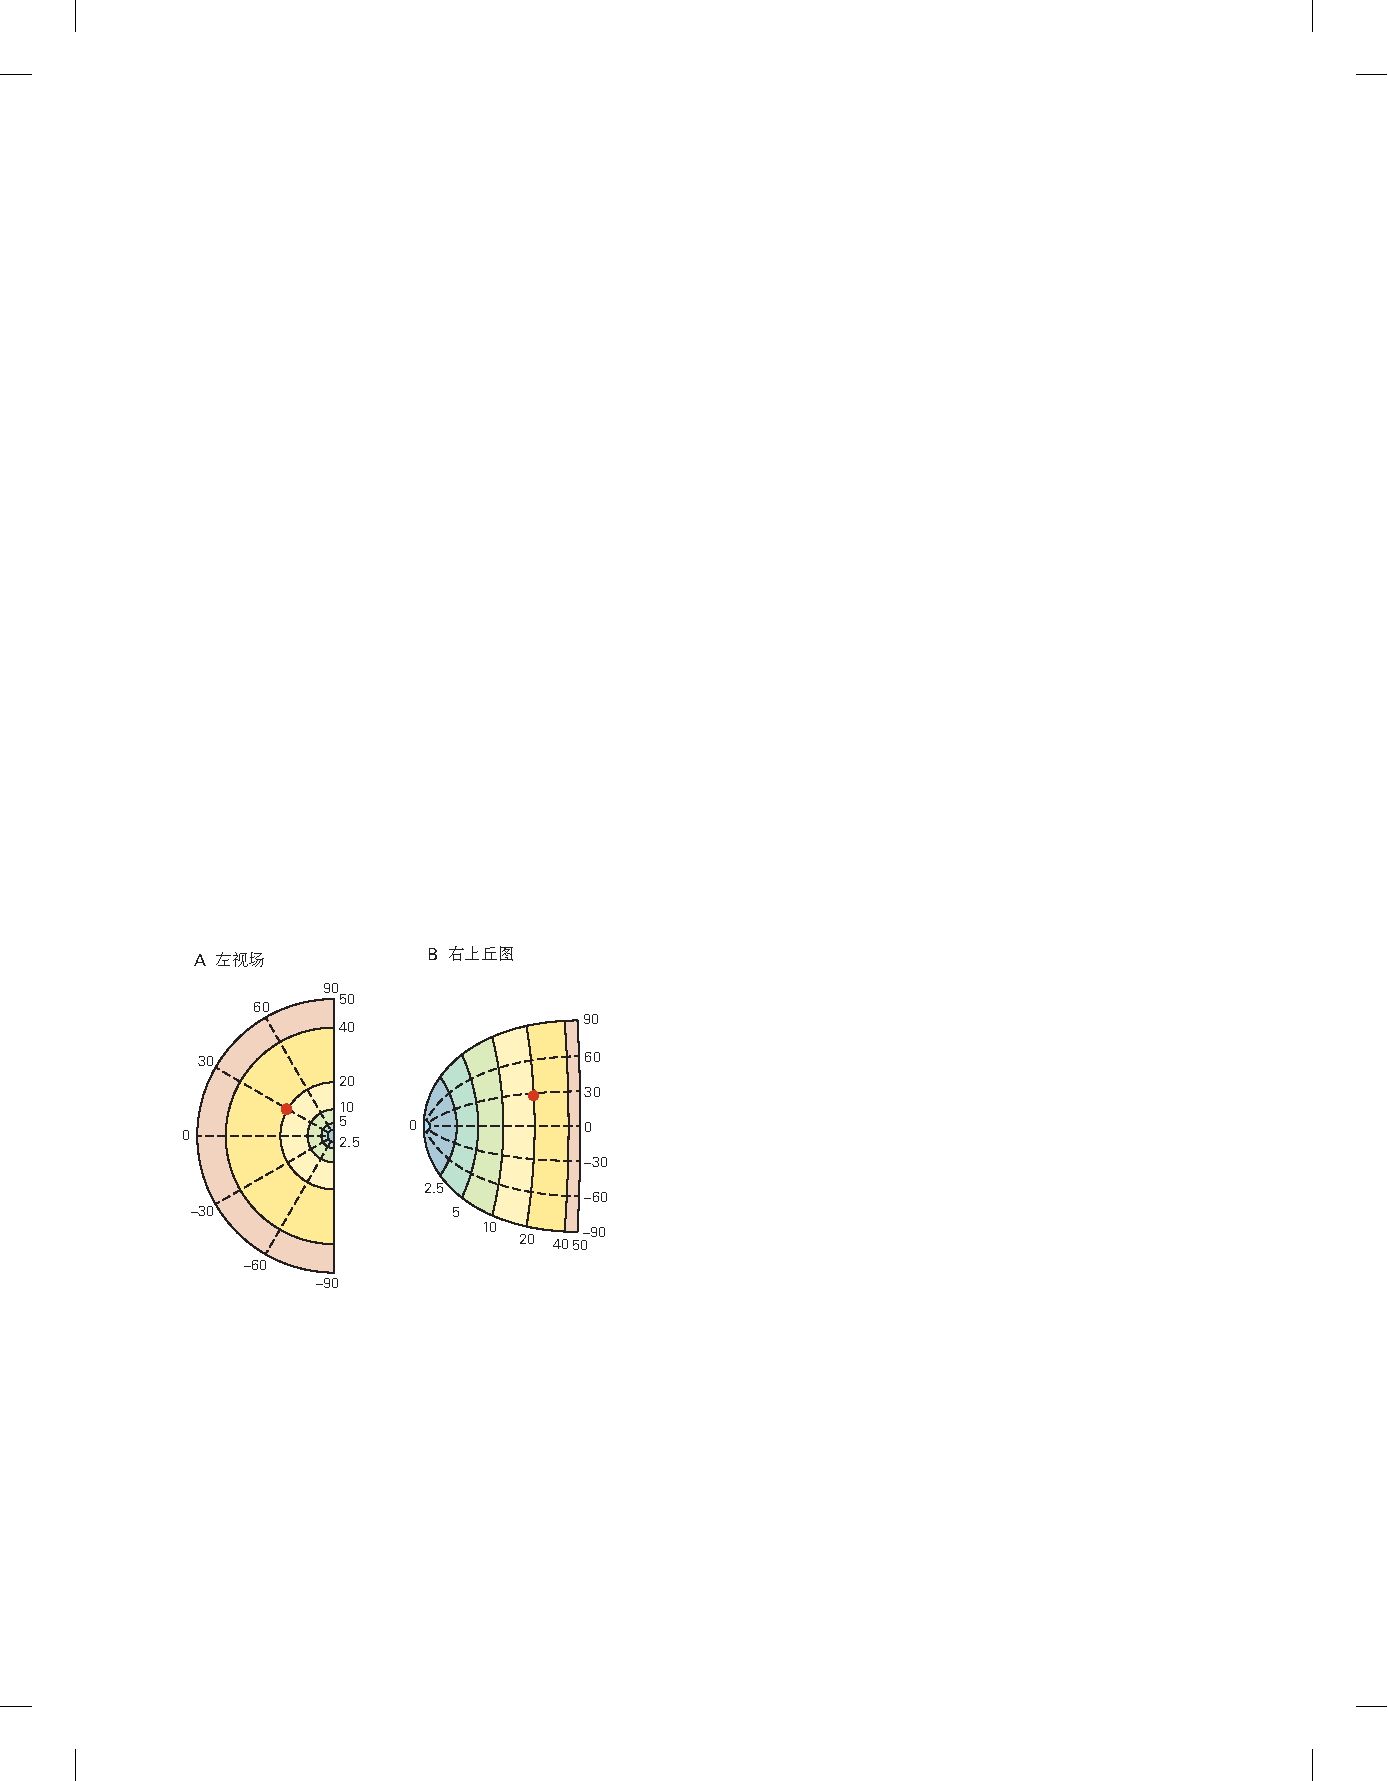
\includegraphics[width=0.5\linewidth]{chap35/fig_35_10}
	\caption{上丘中的神经元组织在视网膜专题图中。 A. 极坐标中左视野图。 虚线代表角度,实线代表偏心率。 B. 以视野极坐标表示的上丘神经元空间图。 在细胞核中,更多的神经元代表靠近中央凹的视野部分,而更少的神经元代表外围。 例如,在视野(红点)中出现 20° 偏心和 30° 仰角的刺激将激发丘地图上红点位置的神经元。 (经许可转载自 Quaia 等人,1998 年。)}
	\label{fig:35_10}
\end{figure}

中间层和深层的神经元活动主要与动眼神经活动有关。 这些层中与运动相关的神经元接收来自前纹状体、中颞叶和顶叶皮质的视觉信息以及来自额叶眼区的运动信息。 中间层和深层还包含感觉输入的躯体图、色调图和视网膜图,所有这些都相互登记。 例如,鸟的图像会激发视觉相关的神经元,而鸟的鸣叫声会激发相邻的听觉相关的神经元,两者都会激发双峰神经元。 多模态空间图使我们能够将眼睛转向听觉或体感刺激以及视觉刺激。

许多描述中间层神经元感觉反应的早期研究都是在麻醉动物身上进行的。 然而,要了解大脑如何产生运动,需要在警觉、活跃的动物身上研究神经元的活动。 爱德华·埃瓦茨 (Edward Evarts) 在骨骼运动系统的研究中开创了这种方法,之后将其扩展到眼球运动系统。

对活跃动物进行的最早细胞研究之一表明,上丘中与运动相关的个体神经元在特定幅度和方向的眼跳之前选择性放电,就像上丘中与视觉相关的个体神经元对来自特定距离和方向的刺激作出反应一样。 中央凹(图 \ref{fig:35_11} A)。 
与运动相关的神经元形成潜在眼球运动的地图,该地图与感觉输入的视位和音位阵列对齐,因此控制眼球运动到特定目标的神经元与被视觉刺激的细胞位于同一区域。 该目标的声音和图像。 上丘中每个与运动相关的神经元都有一个运动场,即视野中的一个区域,是该神经元控制的眼跳的目标。 中间层的运动场图与上覆的表层视觉感受野图对齐。 每个运动神经元在扫视到覆盖的视觉感受野的中心之前放电。 由中间层的电刺激引起的眼跳图类似于视觉图。

\begin{figure}[htbp]
	\centering
	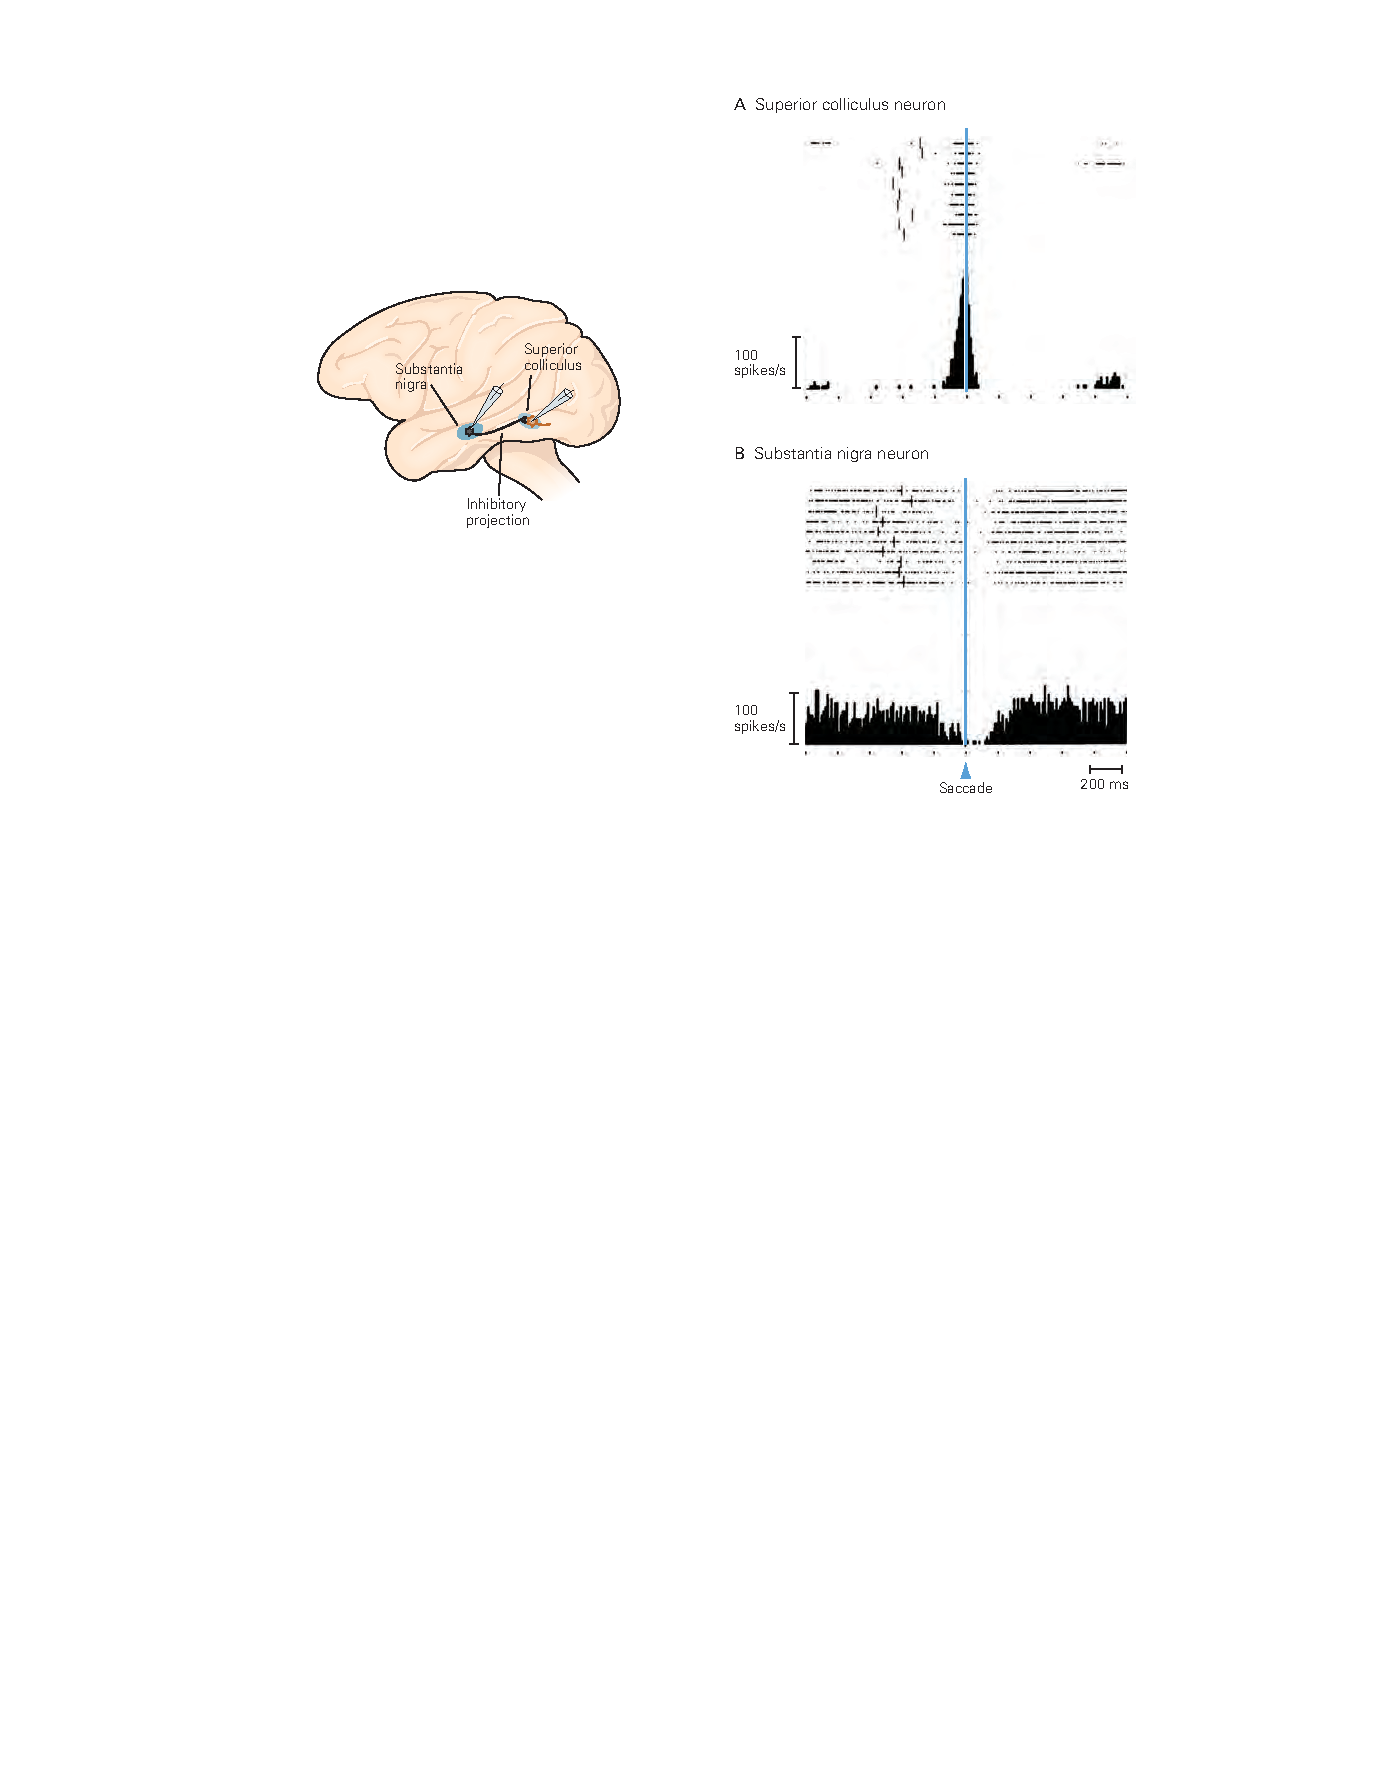
\includegraphics[width=0.5\linewidth]{chap35/fig_35_11}
	\caption{上丘和黑质中的神经元在眼跳前后活跃。 (经许可转载自 Hikosaka 和 Wurtz,1989 年。)A. 从上丘区域记录的神经元,B 中的神经元可以从该区域逆向兴奋,紧接在眼跳之前突然爆发。 同一任务的连续试验中的活动光栅图相加形成下面的直方图。 光栅中的小垂直线表示目标外观。 试验在扫视开始时对齐(蓝线)。 B. 黑质网状部中的一个神经元是紧张活跃的,在眼跳之前变得安静,并在眼跳之后恢复活动。 这种类型的神经元抑制上丘中间层的神经元。}
	\label{fig:35_11}
\end{figure}

运动场很大,因此每个上丘细胞都在大范围的眼跳之前放电,尽管每个细胞在特定方向和幅度的眼跳之前放电最强烈。 因此,在每次扫视之前,大量细胞处于活跃状态,并且眼球运动由这些广泛调谐的细胞的整个集合编码。 由于每个电池对运动的方向和振幅只做出很小的贡献,因此给定电池放电中的任何变化或噪声都被最小化。 在许多感觉系统(第 17 章)和骨骼运动系统(第 34 章)中发现了类似的群体编码。

上丘表层和中间层的活动可以独立发生:表层的感觉活动并不总是导致运动输出,并且运动输出可以在表层没有感觉活动的情况下发生。 事实上,表层的神经元并不直接向中间层提供大的投射。 相反,它们的轴突终止于丘脑枕核和外侧后核的神经元,这些神经元将来自上丘浅层的信号传递到投射回中间层的皮质区域。

一小部分丘的损伤会影响眼跳的潜伏期、准确性和速度。 整个丘的破坏使猴子无法进行任何反向眼跳,尽管随着时间的推移,这种能力会恢复。

\subsection{头侧上丘促进视觉固定}
上丘的最延髓部分接收来自中央凹和初级视觉皮层 (V1) 中的中央凹表示的输入。 该区域中间层的神经元在主动注视期间和对侧视野的小扫视之前强烈放电。 由于神经元在注视过程中很活跃,因此上丘的这个区域通常被称为注视区。

这里的神经元会抑制丘脑尾部与运动相关的神经元,并且还会直接投射到中缝背侧的核,在那里它们通过刺激全停滞神经元来抑制眼跳的产生。 如果注视区有损伤,动物更可能对分散注意力的刺激进行扫视。

\subsection{基底神经节和大脑皮层的两个区域控制上丘}
上丘接收来自黑质神经元的强大的 GABA 能抑制投射,这些神经元以高频率自发放电。 这种放电在自愿眼球运动到对侧视野(图 \ref{fig:35_11} B)时被尾状核中神经元的抑制性输入抑制,尾状核神经元在扫视到对侧视野之前发射。

上丘由大脑皮层的两个区域控制,这两个区域具有重叠但功能不同:后顶叶皮层的外侧顶内区(布罗德曼区 7 的一部分)和额叶眼区(布罗德曼区 8 的一部分)。 这些区域中的每一个都有助于眼跳的产生和视觉注意力的控制。

对视野中有人注意的物体的感知优于对无人注意的物体的感知,这是通过受试者对突然出现在视野中的物体的反应时间或受试者感知几乎不可察觉的刺激的能力来衡量的。 扫视眼球运动和视觉注意密切相关(图 \ref{fig:35_5})。

猴子的侧顶内区域对于视觉注意力和眼跳的产生很重要。 这个区域在处理眼球运动中的作用最好用记忆引导的扫视来说明。 为了演示这种扫视,猴子首先注视一个光点。 一个物体(刺激)出现在神经元的感受野中,然后消失; 然后光点熄灭。 延迟一段时间后,猴子必须对消失物体的原位置进行扫视。 
外侧顶内区域的神经元从物体出现的那一刻开始响应,并在物体消失后继续放电,并在整个延迟期间一直持续到眼跳开始(图 \ref{fig:35_12}A),但它们的活动也可以与眼跳计划分离。 
如果猴子计划对神经元感受野外的目标进行扫视,并且在延迟期间干扰物出现在视野中,神经元对干扰物的反应与对扫视目标的反应一样强烈(图 \ref{fig:35_12} B).

\begin{figure}[htbp]
	\centering
	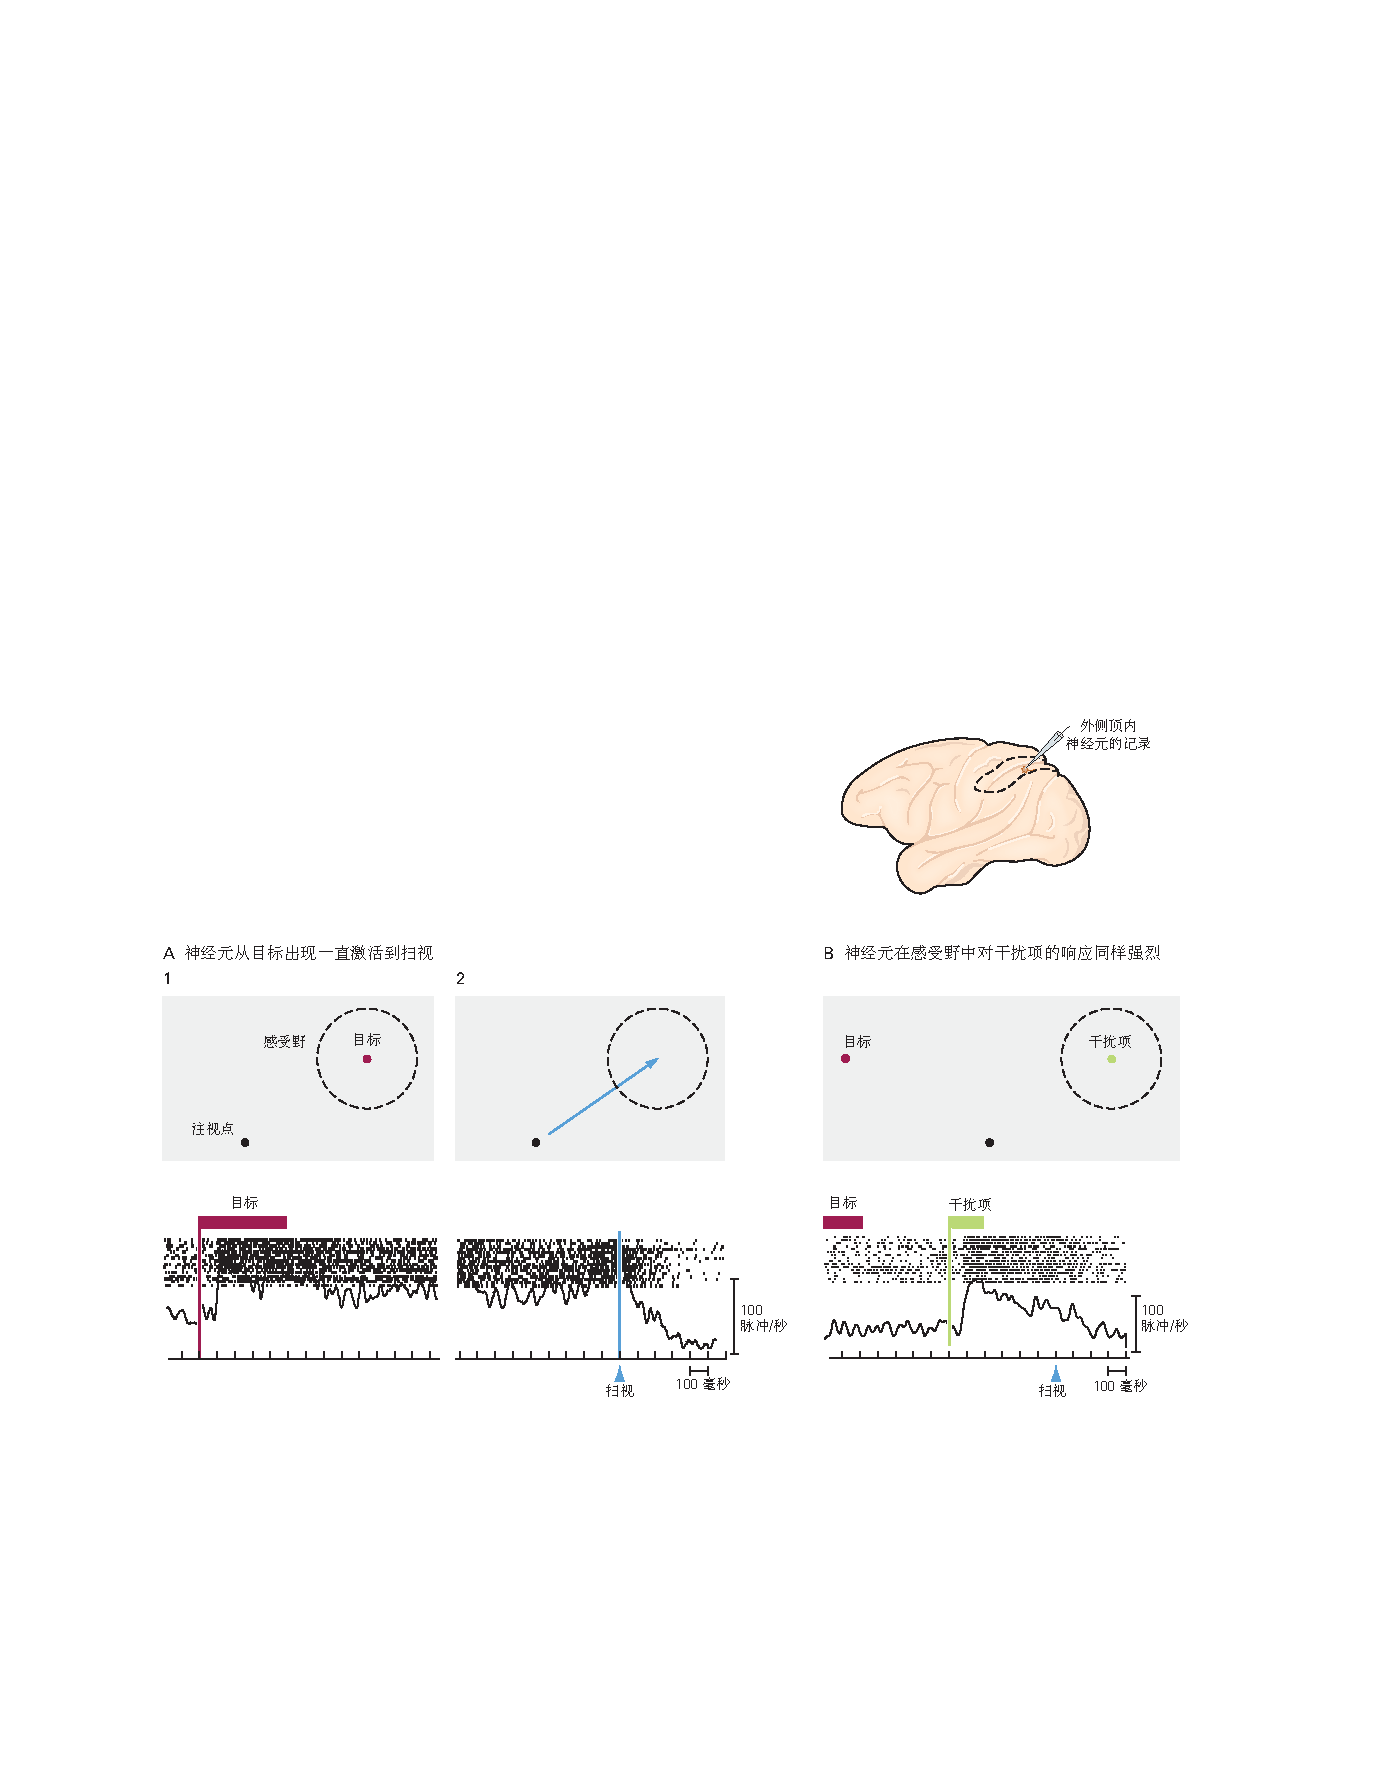
\includegraphics[width=0.95\linewidth]{chap35/fig_35_12}
	\caption{顶叶神经元在记忆引导的扫视之前活跃。 跟踪在垂直线指示的事件处对齐。 (经许可改编自 Powell 和 Goldberg 2000。) A. 猴子计划从注视点到外侧顶内皮层神经元感受野中的目标进行扫视。 神经元响应目标 (1) 的出现。 它在目标消失后但在发出扫视信号之前继续发射,并在扫视开始后停止发射 (2)。 B. 猴子计划对感受野外的目标进行扫视。 神经元最初对感受野中的干扰物的反应与对扫视目标的反应一样强烈。}
	\label{fig:35_12}
\end{figure}

猴子的后顶叶皮层(包括外侧顶内区域)的损伤会增加眼跳的潜伏期并降低其准确性。 这种损伤也会产生选择性忽视:单侧顶叶损伤的猴子优先注意同侧视觉半场的刺激。 同样在人类中,顶叶病变——尤其是右顶叶病变——最初会导致严重的注意力缺陷。 患者表现得好像被忽视的领域中的物体不存在,并且他们很难将眼球移动到那个领域(第 59 章)。

Balint 综合征患者通常是后顶叶皮层和前纹状皮层双侧损伤的结果,往往在他们的视觉环境中一次只能看到和描述一个物体。 这些患者很少进行扫视,就好像他们无法将注意力从中央凹转移开一样,因此只能描述中央凹目标。 即使在这些患者从大部分缺陷中恢复过来之后,他们的眼跳仍会延迟且不准确。

与顶叶皮层中的神经元相比,额叶眼区中的神经元与眼跳更为密切相关。 额叶眼区的三种不同类型的神经元在扫视前放电。

视觉神经元对视觉刺激作出反应,这些神经元中有一半对眼跳目标的刺激反应更强烈(图 \ref{fig:35_13}A)。 
当动物对刺激做出反应而不进行扫视时,这些细胞的活动不会增强。 同样,在没有视觉目标的情况下进行的扫视之前,这些细胞不会被激活; 可以训练猴子在完全黑暗中进行特定方向和振幅的扫视。

\begin{figure}[htbp]
	\centering
	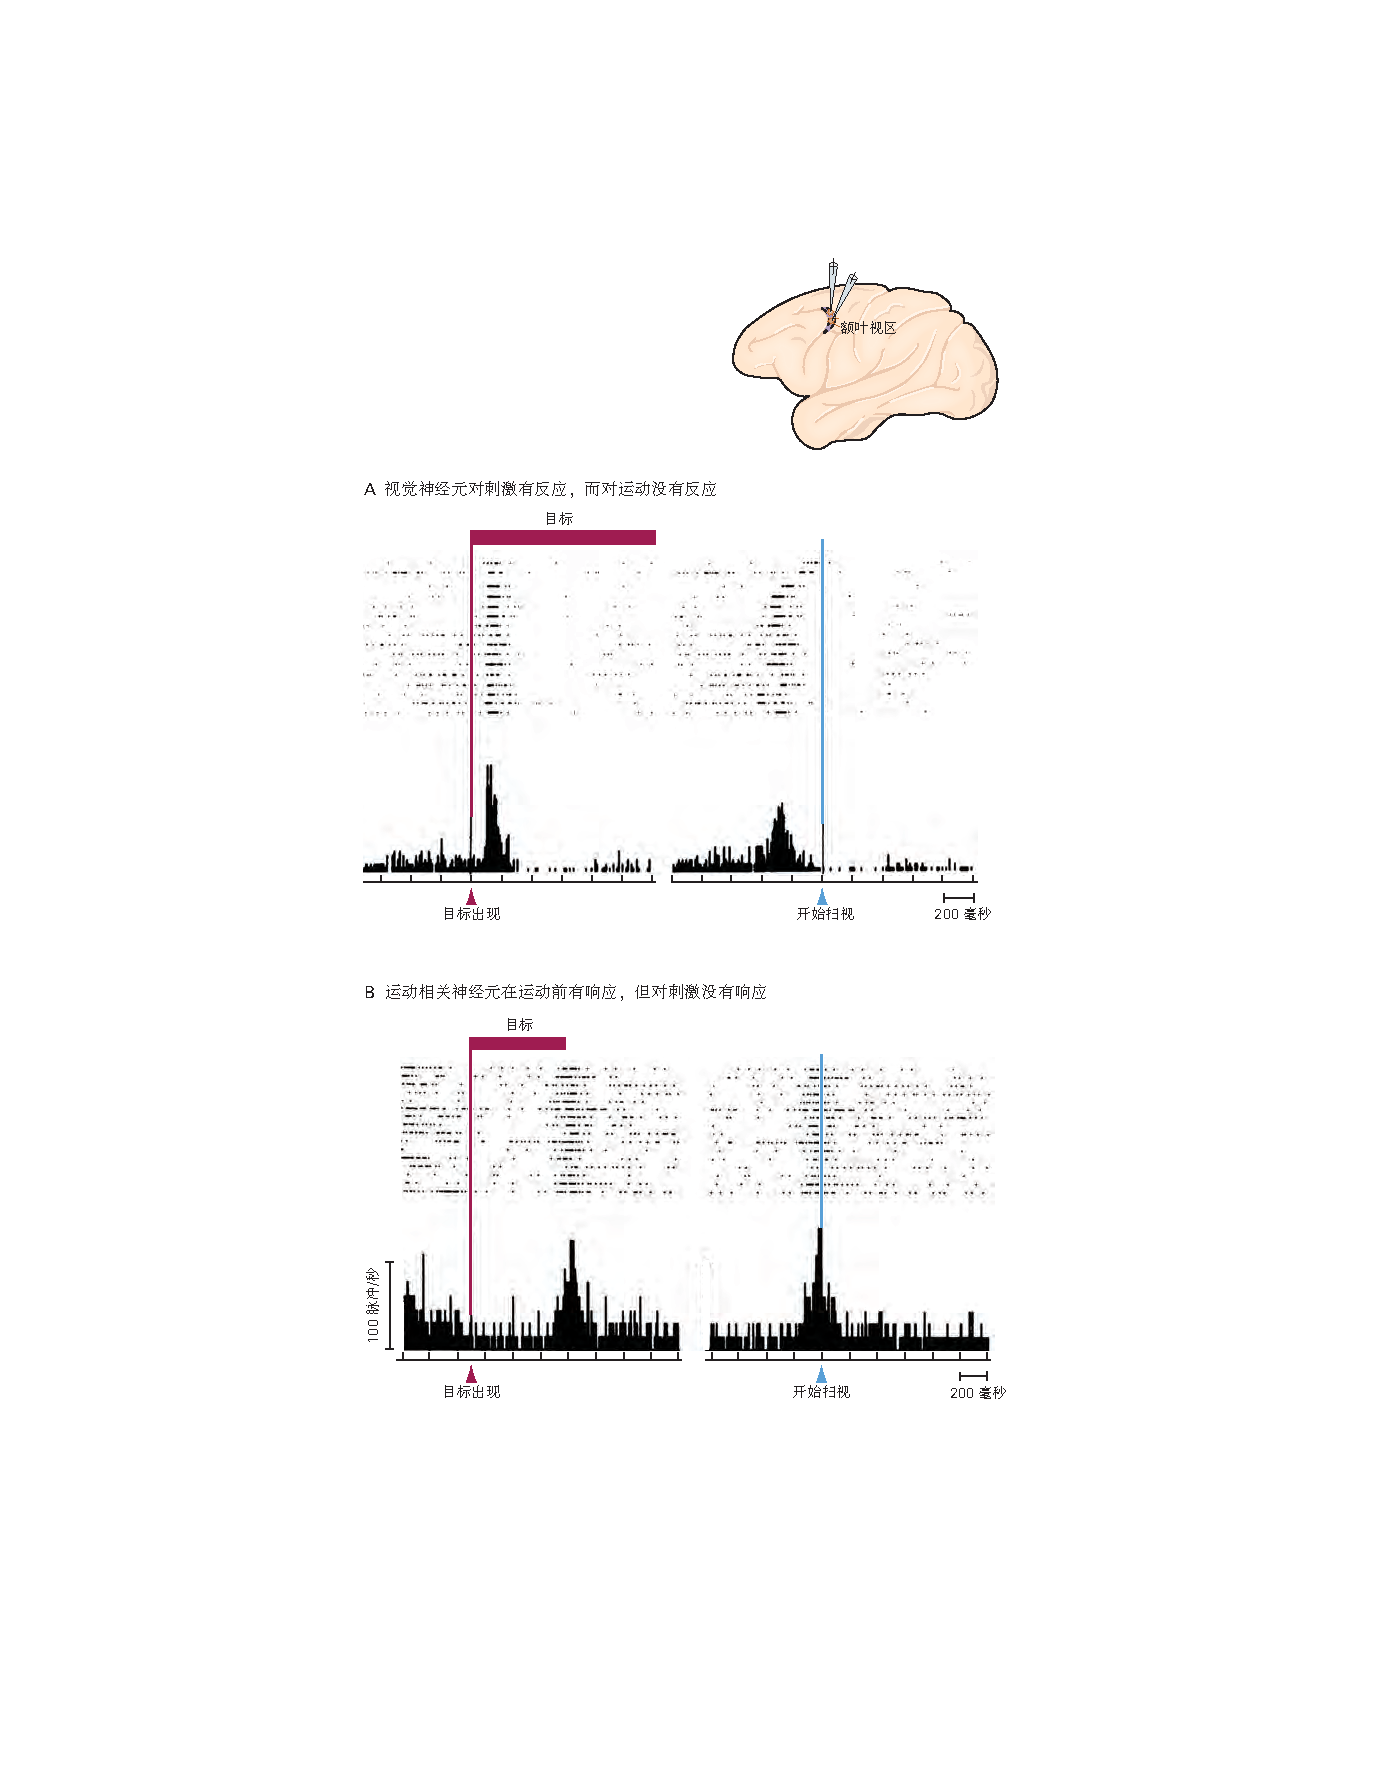
\includegraphics[width=0.65\linewidth]{chap35/fig_35_13}
	\caption{额眼区的视觉和运动相关神经元。 (经许可转载自 Bruce 和 Goldberg 1985。) A. 当猴子对视野中的目标进行扫视时,额眼区视觉神经元的活动。 同一任务的连续试验中的活动光栅图相加形成下面的直方图。 在左侧的记录中,各个试验在刺激出现时对齐。 一阵射击与刺激密切相关。 在右侧的记录中,试验在扫视开始时对齐。 活动与扫视的开始并没有很好地对齐,并且在扫视本身开始之前就停止了。 B. 额眼区运动相关神经元的活动。 每个试验的记录都按照 A 部分对齐。细胞对扫视目标(左)的出现没有反应,但在扫视时处于活动状态(右)。}
	\label{fig:35_13}
\end{figure}

与运动相关的神经元在扫视运动场之前和期间会放电。 与在所有眼跳之前激活的上丘中的运动相关细胞不同,额眼场的运动相关神经元仅在与猴子行为相关的眼跳之前激活(图 \ref{fig:35_13} B)。 这些神经元,尤其是那些感受野位于视觉周边的神经元,比视觉神经元更强烈地投射到上丘。

视觉运动神经元具有视觉和运动相关的活动,并且在视觉引导的扫视之前放电最强烈。 额叶眼场的电刺激会引起对受刺激细胞运动场的扫视。 额叶眼场的双侧刺激引起垂直扫视。

额叶眼区的运动相关神经元通过两条途径控制上丘。 它们直接刺激上丘,并通过刺激尾状核将其从黑质的抑制影响中释放出来,而尾状核又反过来抑制黑质(图 \ref{fig:35_9} A)。 额叶视野也投射到脑桥和中脑网状结构,但不直接投射到爆裂细胞。

除了 LIP 之外,另外两个皮层区域对额叶眼场有输入,被认为在扫视的认知方面很重要。 辅助运动区最前端部分的辅助眼区包含编码空间信息的神经元,而不是所需眼球运动的方向。 例如,如果左眼扫视是在目标的右侧,通常在右眼运动之前发射的左辅助眼区中的神经元将在左眼扫视之前发射。 背外侧前额叶皮层的神经元会在猴子向记住的目标扫视时放电。 活动从刺激的出现开始,并在猴子必须记住目标位置的整个时间间隔内持续进行。

我们现在可以了解这些区域的损伤对眼跳产生的影响。 猴子上丘的损伤只会对眼跳系统造成短暂的损伤,因为从额叶视野到脑干的投射仍然完好无损。 如果上丘完好无损,动物同样可以从皮质损伤中恢复过来。 然而,当额叶视野和丘都受损时,眼跳的能力就会永久受损。 顶叶病变的主要影响是注意力缺陷。 然而,恢复后,系统可以正常工作,因为额叶眼场信号足以抑制黑质并刺激丘。

仅额叶眼区的损伤会导致更细微的缺陷。 猴子额眼区的损伤会导致短暂的对侧忽视和逆向凝视麻痹,这些都会迅速恢复。 后一种缺陷可能反映了黑质额叶眼区控制的丧失; 这种失控意味着从黑质到丘的持续抑制性输入没有受到抑制,丘无法产生任何眼跳。 最终系统适应,丘对剩余的顶叶信号做出反应。 恢复后,这些动物可以毫无困难地对视野中的目标进行扫视,但在记忆引导的扫视中却有很大困难。 额叶视野和上丘的双侧损伤使猴子根本无法进行眼跳。

额叶皮层受损的人很难抑制不需要的眼跳以注意刺激。 这很容易通过要求受试者将眼球从刺激物上移开来证明,即“反扫视任务”。 例如,如果左侧出现刺激,则受试者应向右侧进行相同大小的扫视。 为此,受试者必须注意刺激,而不是将眼睛转向它,并使用它的位置来计算所需的向相反方向的扫视。 额叶病变患者很难抑制对刺激的不希望的扫视。

正如我们所见,当动物注意到视觉刺激时,无论动物是否对刺激进行扫视,猴子外侧顶内区域的神经元都会活跃。 在没有额叶眼场信号的情况下,这种未分化的信号是唯一到达上丘的信号。 因此,在人类中,如果上丘对产生对刺激的注意力的顶叶信号作出反应而没有额叶-黑质控制通常会阻止响应顶叶信号的眼跳,则可以预期无法抑制眼跳。

\subsection{扫视的控制可以通过经验来修改}
运动神经控制的定量研究是可能的,因为运动神经元的放电率对运动有可预测的影响。 例如,外展运动神经元的特定频率放电对眼睛位置和速度具有可预测的影响。

如果疾病损害动眼神经或导致眼部肌肉变弱,这种关系可能会发生变化,尽管大脑可以在某种程度上补偿这种变化。 Guntram Kommerell 描述了一个案例,戏剧性地说明了这一点。 一名糖尿病患者的一只眼睛出现急性部分外展神经损伤,另一只眼睛出现视网膜出血。 由于外展神经正常的眼睛视力不佳,他通常使用新近削弱的外直肌的眼睛。 几天后,眼睛恢复了相当准确的眼球运动能力。 当弱眼被修补并且受试者试图用视力不佳的眼睛进行扫视时,扫视超出了目标。 这意味着为了补偿视觉正常眼睛的弱点,大脑增加了双眼的神经信号,导致正常运动输入的眼睛信号过大。 运动反应的这种变化取决于小脑的顶核和蚓部(图 \ref{fig:35_9} A),并且是视觉系统发出信号表明之前的眼球运动不准确的结果。

\subsection{一些快速的视线转移需要协调的头部和眼睛运动}
到目前为止,我们已经描述了当头部静止时眼睛是如何移动的。 然而,当我们环顾四周时,我们的头也在移动。 必须协调头部和眼睛的运动以将中央凹引导至目标。

因为头部的惯性比眼睛大得多,所以在头部开始移动之前,注视的微小变化会驱使中央凹到达目标。 
一个小的注视转移通常包括一个扫视,然后是一个小的头部运动,在此期间,前庭眼反射将眼睛移回新头部位置的眼眶中心(图 \ref{fig:35_14})。 
对于较大的凝视移动,眼睛和头部同时向同一方向移动。 由于前庭眼反射通常使眼睛向与头部相反的方向移动,因此必须暂时抑制反射。

\begin{figure}[htbp]
	\centering
	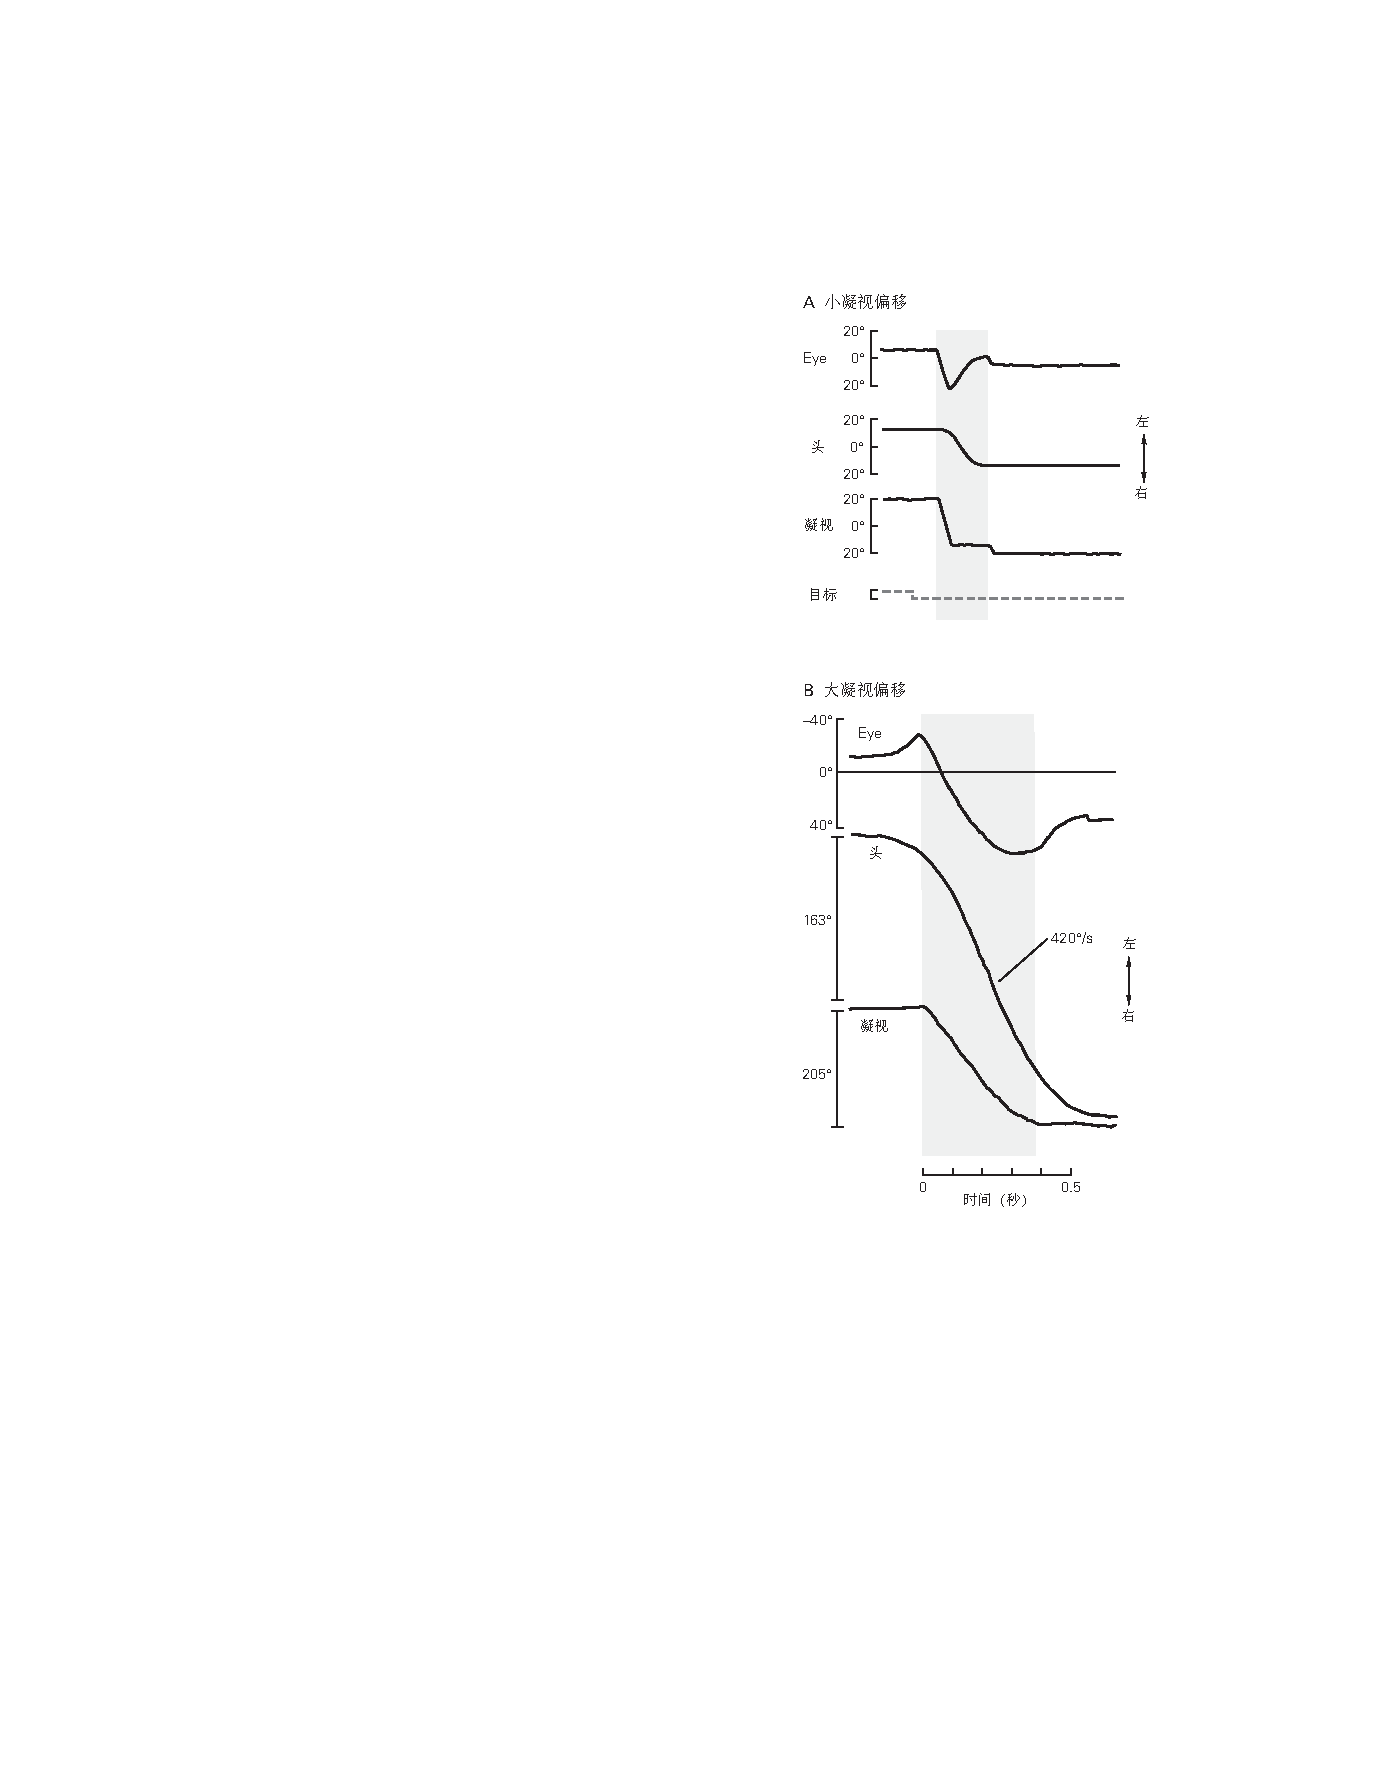
\includegraphics[width=0.4\linewidth]{chap35/fig_35_14}
	\caption{}
	\label{fig:35_14}
\end{figure}


\section{平滑跟踪系统保持移动的目标在中央凹上}
平滑追踪系统通过计算目标移动的速度和眼睛以相同速度移动的速度,将移动目标的图像保存在中央凹上。 平滑追踪运动的最大角速度约为每秒 100°,比扫视慢得多。 药物、疲劳、酒精甚至分心都会降低这些运动的质量。

平滑追踪和扫视具有截然不同的中央控制系统。 当目标从注视中心跳开然后慢慢移回注视中心时,这种情况最为明显。 首先启动平滑追踪运动,因为平滑追踪系统具有较短的延迟并且响应周边视网膜和中央凹上的目标运动。 平滑追踪系统的任务不同于扫视系统。 它不是将眼睛尽可能快地驱动到空间中的一个点,而是必须使眼睛的速度与空间中目标的速度相匹配。 因此,当目标移回注视中心时,平滑追踪系统会在扫视开始前短暂地将眼睛从目标移开(图 \ref{fig:35_6}B)。 随后的扫视将眼睛带到目标上。 在前庭内侧核和舌下前核中发现了发出眼球速度信号以进行平稳追踪的神经元。 它们接收来自小脑绒球的投射,并投射到外展核以及中脑的动眼神经核。

绒球和蚯蚓中的神经元传输与平稳追踪相关的眼速信号。 
这些区域接收由脑桥背外侧核中继的大脑皮层信号(图 \ref{fig:35_15})。
因此,背外侧脑桥的损伤会破坏同侧的平稳追踪。

\begin{figure}[htbp]
	\centering
	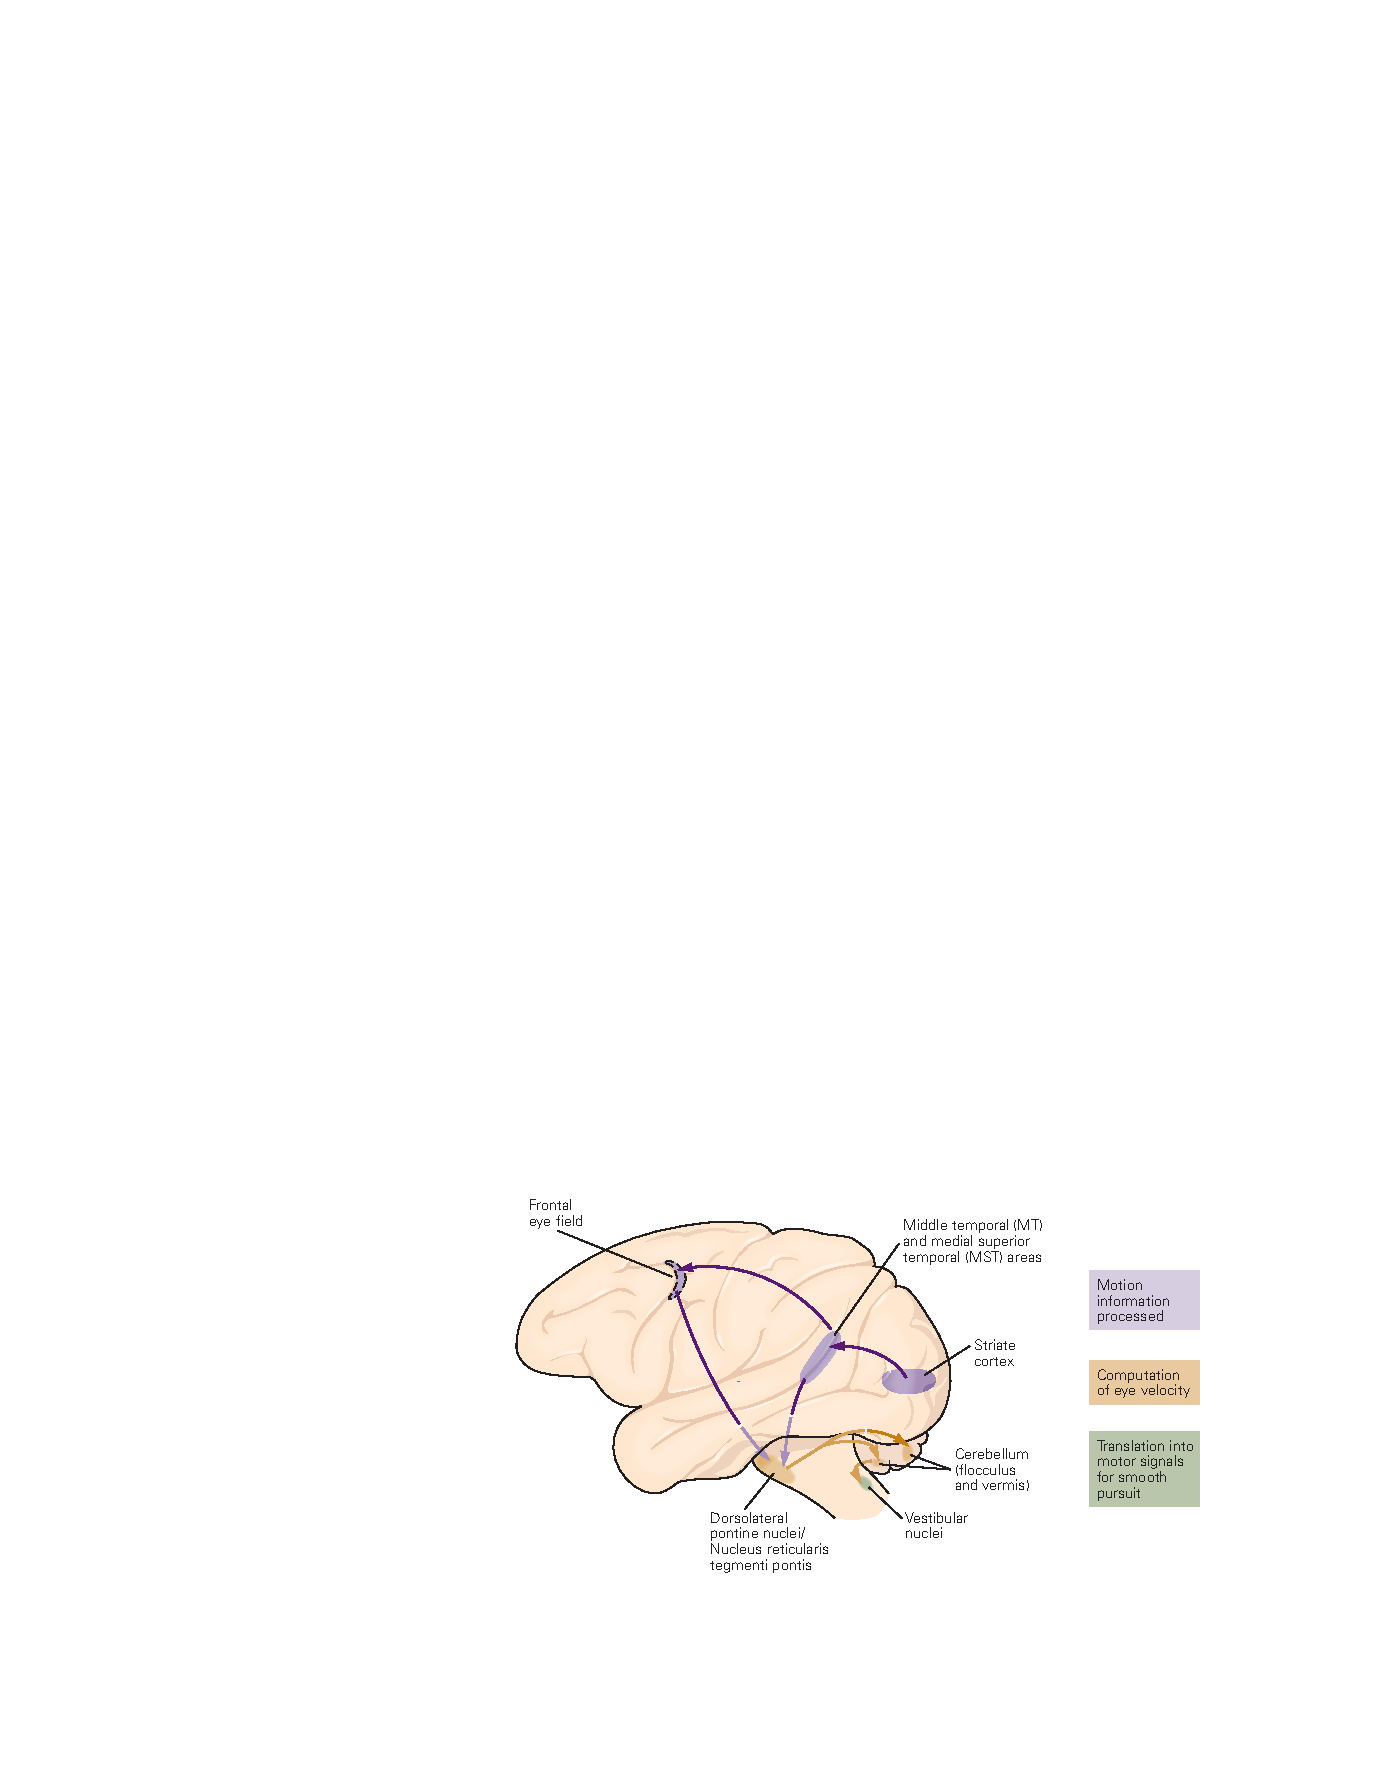
\includegraphics[width=0.7\linewidth]{chap35/fig_35_15}
	\caption{猴子平滑追踪眼球运动的皮质通路。 大脑皮层处理有关视野中运动的信息,并通过背外侧脑桥核、小脑蚓部和绒球以及前庭核将其发送到动眼神经元。 平稳追踪的启动信号可能部分源自额眼区。}
	\label{fig:35_15}
\end{figure}

猴子的 smoothpursuit 系统有两个主要的皮层输入。 一种起源于颞上沟、颞中部和内侧颞上区的运动敏感区。 另一个来自额眼区。

中颞区和内侧上颞区因其位于猫头鹰猴(一种新世界猴)的无沟皮质中而得名。 在人类和旧世界猴子中,这些区域位于颞上沟,在枕叶和顶叶之间的交界处。 中颞区和内侧上颞区的神经元计算目标的速度。 当眼睛加速以匹配目标的速度时,目标在视网膜上的运动速率会降低。 随着视网膜图像速度的降低,中间颞区的神经元(其活动发出视网膜图像运动信号)停止放电,即使目标继续在空间中移动也是如此。 即使目标短暂消失,内侧上颞区的神经元也会继续放电。 这些神经元可以访问一个过程,该过程将移动眼睛的速度和目标在视网膜上移动的速度相加,以计算目标在空间中的速度。

中颞区或内侧上颞区的损伤会破坏受试者对在受损皮质区域代表的视野区域中移动的目标做出反应的能力。 无论目标位于视网膜上的哪个位置,后一区域的病变也会减少向病变一侧的平滑追踪运动。

这两个运动选择区域提供感官信息来指导追逐运动,但可能无法启动它们。 任一区域的电刺激都不会启动平稳的追逐,但可以影响追逐运动,加速同向追逐并减慢反向追逐。 正面视野对于发起追逐可能更为重要。 该区域的神经元会随着同向的平稳追逐而发射。 额叶眼场的电刺激启动同向追逐,而该区域的病变减少但不消除平滑追逐。

在人类中,追踪路径沿途任何地方的中断,包括皮质、小脑和脑干区域水平的损伤,都会阻止足够的平滑追踪眼球运动。 相反,使用有缺陷的平滑追踪运动(速度小于目标速度)和小扫视的组合来跟踪移动目标。 脑干和小脑病变的患者不能追求向病变一侧移动的目标。

包括运动敏感区域在内的顶叶缺陷患者有两种不同类型的缺陷。 第一个是方向性缺陷,类似于患有内侧颞上区病变的猴子:无法追踪向病变一侧移动的目标。 第二种是类似于患有中颞区病变的猴子的视黄质缺陷:无论运动方向如何,都存在对仅限于病变对面的视觉半视野的刺激的平稳追求的损害。


\section{聚散系统将眼睛对齐到不同深度的目标上}
平滑追踪和扫视系统产生共轭眼球运动:双眼以相同的方向和相同的速度移动。 相反,聚散系统产生眼睛的非共轭运动。 当我们注视一个离我们很近的物体时,我们的眼睛会聚或向对方转动; 
当我们看一个更远的物体时,它们会发散或旋转远离彼此(图 \ref{fig:35_16})。 
这些分离运动确保物体的图像落在两个视网膜的中央凹上。 视觉系统利用左右视网膜位置的细微差异或视网膜视差来产生深度感,而聚散运动则消除中央凹处的视网膜视差。

\begin{figure}[htbp]
	\centering
	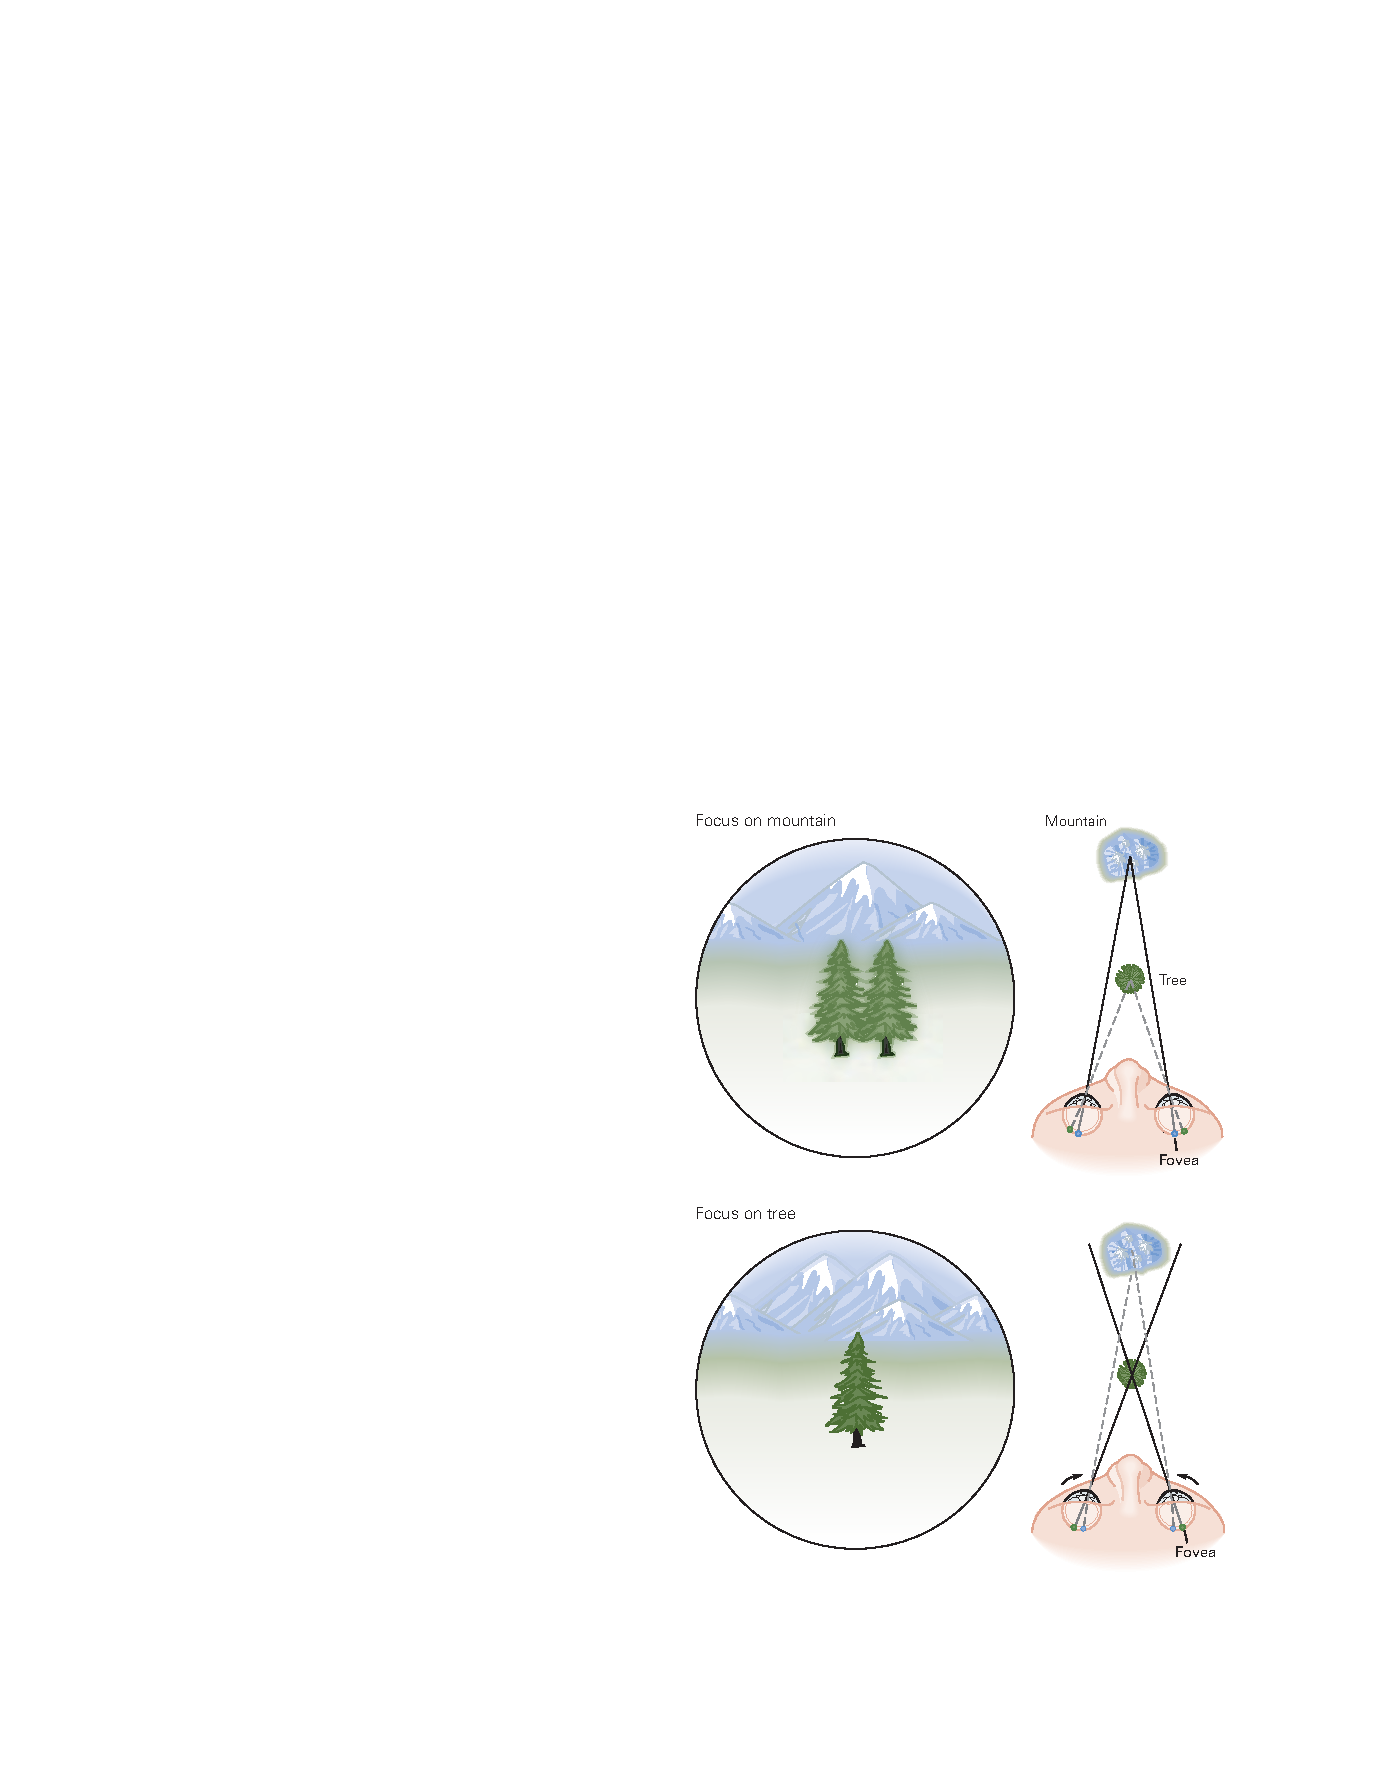
\includegraphics[width=0.65\linewidth]{chap35/fig_35_16}
	\caption{辐辏运动。 当眼睛注视远处的山时,山的影像位于中央凹,而前方树木的影像占据不同的视网膜位置,产生双重影像的感知。 当观察者转而注视树时,聚散系统必须将每只眼睛向内旋转。 现在,树的图像在两个中央凹上占据相似的位置,并被视为一个物体,但山的图像在视网膜上占据不同的位置,看起来是双重的。 (经许可转载自 F.A. Miles。)}
	\label{fig:35_16}
\end{figure}

聚散度仅是水平直肌的功能,因为两只眼睛是水平而非垂直移位的。 用于近场观看的眼睛会聚是通过同时增加内侧直肌的张力和降低外侧直肌的张力来使眼睛会聚来实现的。 相反,远距离观察是通过降低内直肌的张力和增加外直肌的张力来实现的。

在任何给定时间,整个视野都不会聚焦在视网膜上。 当我们看近处的东西时,远处的物体是模糊的。 当我们看远处的东西时,近处的物体是模糊的。 当我们希望聚焦在视野中较近平面中的物体时,动眼神经系统收缩睫状肌,从而改变晶状体的曲率半径。 这个过程称为适应。 随着年龄的增长,由于晶状体硬度增加,调节能力下降; 然后需要老花镜来聚焦近距离的图像。

住宿和聚散度是相关的。 调节是由图像的模糊引起的,每当调节发生时,眼睛也会聚集。 相反,视网膜差异会引起聚散,每当眼睛会聚时,也会发生调节。 同时,瞳孔会暂时收缩以增加焦点的景深。 调节、聚散和瞳孔收缩的相关现象构成了近距离反应。 调节和聚散由动眼神经核区域的中脑神经元控制。 该区域的神经元在聚散、调节或两者同时放电。



\section{要点}
1. 动眼神经系统为临床医生和科学家提供了了解神经系统的宝贵窗口。 患有动眼神经缺陷的患者可能会出现复视等令人担忧的症状,这些症状会使他们迅速寻求医疗帮助。 对动眼神经系统有透彻了解的医生可以在床边描述和诊断大多数动眼神经缺陷,并根据眼球运动的神经解剖学和神经生理学定位大脑内的病变部位。

2. 眼球运动的目的是在眼眶中转动眼球,以便将中央凹(视网膜上具有最佳敏锐度的区域)引导到视觉场景中最感兴趣的点,然后保持图像稳定。

3. 六块肌肉共同作用来移动每只眼睛。 这些眼部肌肉分为三对。 外直肌水平外展眼球,内直肌内收眼球。 旋转眼肌在垂直方向和扭转方向上移动眼睛。

4. 眼外肌的运动神经元位于三个脑干核团中。 脑桥中的外展核包含外直肌的神经元。 其他动眼神经元位于中脑:滑车核包含上斜神经元,动眼神经核包含内侧、上、下直肌和下斜肌的运动神经元。 收缩瞳孔和抬高眼睑的神经元也位于动眼神经核中。

5. 有六种不同类型的眼球运动,具有不同的控制系统: (1) 眼跳快速将中央凹转移到新的视觉目标。 (2) 平滑追踪运动将移动物体的图像保留在中央凹上。 (3) 聚散运动使眼睛向相反的方向旋转,以便无论距离多远,感兴趣的物体的图像都位于两个中央凹上。 (4) 前庭眼反射在短暂、快速的头部运动期间将图像保持在视网膜上。 (5) 视动运动在持续或缓慢的头部运动期间保持图像静止。 (6)注视是在头部不动时,在注视过程中保持眼睛静止的主动过程。

6. 眼肌神经元的放电模式结合了编码眼睛位置和速度的独立信号。 产生水平扫视速度信号的神经元位于桥脑旁正中网状结构中,该速度信号整合在内侧前庭核和舌下核前置核中以提供位置信号。

7. 中脑网状结构为垂直和扭转眼球运动以及聚散眼球运动提供位置和速度信号。

8. 上丘中的 Presaccadic burst 神经元将所需的位移信号投射到网状结构。 这些神经元被来自黑质的 GABAergic 投射抑制,并被来自额叶视野和后顶叶皮层的投射兴奋。 来自额叶眼场的运动信号激发尾状核,然后尾状核抑制黑质,使眼跳发生。

9. 后顶叶皮层向上丘投射注意信号,不区分注意和运动。

10. 大多数大的凝视转移都涉及头部运动和眼球运动。 因为眼睛比头移动得快,所以它通常先到达目标。 前庭眼反射通过以与头部运动的速度相反的速度驱动眼睛来保持眼睛在目标上。

11. 小脑根据视觉反馈校准眼球运动并调节学习过程,使它们随着时间的推移保持准确。

12. 平滑追踪是由一个网络驱动的,该网络包括内侧前庭核、小脑绒球、背外侧脑桥核,以及在一些猴子的颞上沟中发现的两个运动选择区域——颞中和内侧 上颞区。 人脑中的同源区域位于顶枕叶交界处。 额眼区的追逐区域启动平滑追逐运动。

13. 尽管眼球运动的运动程序已广为人知,但该领域的大部分生理学研究都是通过猴子对光点进行定向扫视来完成的。 我们对探索视觉世界时自由选择眼跳目标的神经机制知之甚少。 这个位于认知和运动控制交叉点的问题是神经科学中最大的未知数之一,将成为未来动眼神经研究的中心。


\subsection{选读}
\subsection{参考文献}


